The end of the previous chapter presented the $\pi$-POMDPs, 
a qualitative possibilistic counterpart of the classical probabilistic POMDPs.
Recall that, in the qualitative possibilistic framework, the set of belief states is finite, 
$\# \Pi^{\mathcal{S}}_{\mathcal{L}} < +\infty$ (see Equation \ref{equation_numberOfPossDistrib})
while the set of belief states is infinite in the probabilistic framework $\mathbb{P}^{\mathcal{S}}_{b_0}$:
for this reason, $\pi$-POMDPs can be seen as a simpler model 
for sequential decision making under uncertainty,
than the probabilistic one. This is a good point as solving probabilistic POMDPs 
is at least a PSPACE problem \cite{Papadimitriou:1987,Madani:1999:UPP:315149.315395}.
Moreover, Qualitative Possibility Theory allows to model total ignorance
as noted in Introduction: it is a motivation for the study of this model.
The distribution $\forall s \in \mathcal{S}$, $\beta(s) = 1$ means that all
states are plausible according to the belief state $\beta$, \textit{i.e.} 
the agent considers that all system states are possible. 
Finally, possibility distributions only sort events
and represent their plausibility only roughly:
no quantitative value is assigned to them.
If the probability distributions defining the POMDP are not known in practice,
as in the robotic vision example given in Introduction,
a qualitative description of the problem is more suitable.

The pessimistic version of the $\pi$-POMDP model 
has been previously defined in \cite{Sabbadin:1999:pipomdp}.
This section is then devoted to the update of this promising model:
first, optimistic and pessimistic models 
with intermediate preferences are built and discussed.
This discussion leads to other criteria.
Next, the \textit{Mixed-Observability} property \cite{OngShaoHsuWee-IJRR10,AraThoBufCha-ICTAI10} 
is defined, describing the systems some state variables 
of which are fully observable:
it is shown that this property, if correctly taken into account,
dramatically reduces the complexity of solving $\pi$-POMDPs.
Finally, a value iteration algorithm for the infinite horizon 
$\pi$-MDPs (Fully and Partially Observable) 
is next proposed and the optimality of the returned strategy (for a specified criterion) 
is shown assuming the existence of a ``stay'' action in some goal states.
Experimental work finally 
illustrates the performance of the strategies 
computed from different criteria. 
It is also shown that strategies computed 
from $\pi$-POMDPs can
outperform probabilistic POMDP strategies 
for a target recognition problem 
where the agent's observations are imprecise. 

\section{Intermediate Preferences in $\pi$-POMDPs}
In the previous chapter, 
$\pi$-MDPs criteria 
taking into account 
intermediate preference degrees
have been defined;
after that, the particular case 
of terminal preferences only 
has been presented. 
The global preference degree of a trajectory $\mathcal{T} = (s_0,\ldots,s_{H}) \in \mathcal{S}^{H+1}$ 
has been defined there as the minimum of all the preference degrees of the encountered states:
\begin{equation}
\label{globalprefmin2}
 \rho\Big(\mathcal{T},(a_t)_{t=0}^{H-1}\Big) = \min \set{ \min_{t=0}^{H-1} \rho_t\Big(s_t,a_t\Big), \Psi(s_H) }. 
\end{equation}
Another global preference based on the $\max$ operator can be also proposed. 
Let us explicitly define the global preferences for system states:
they are the possibilistic counterparts 
of the sum $\sum_{t = 0}^{H-1} r_t\Big( s_t, a_t \Big) + R(s_H)$ 
in the probabilistic model, given in the equation (\ref{criterion}).  
\begin{Def}[Global Preferences on System State Trajectory]
\label{def_globaldef}
Let $(A_t)_{t=0}^{H-1}$ be a sequence of action variables modeling the successive agent decisions.
Global preferences over system state trajectories $(S_t)_{t=0}^{H}$ are denoted as follows:
\begin{itemize}
\item the \textbf{maximum-based} one, not very demanding,
\begin{equation}
\label{globalprefmax}
\overline{\mathcal{G}} \Big( (S_t)_{t=0}^{H}, (A_t)_{t=0}^{H-1} \Big) = \max \bigg\{ \max_{t=0}^{H-1} \set{ \rho_t\Big( S_t, A_t \Big)  }, \Psi(S_H) \bigg\}, 
\end{equation}
\item the classical \textbf{minimum-based} one, which has been used until now,
\begin{equation}
\label{globalprefmin}
\underline{\mathcal{G}} \Big( (S_t)_{t=0}^{H}, (A_t)_{t=0}^{H-1} \Big) = \min \bigg\{ \min_{t=0}^{H-1} \set{ \rho_t\Big( S_t, A_t \Big)  }, \Psi(S_H) \bigg\},
\end{equation}
\end{itemize}
 \textit{i.e.} with previous notations, 
if the system state trajectory is denoted by $\mathcal{T} = (s_0,\ldots,s_{H}) \in \mathcal{S}^{H+1}$
and the strategy $(\delta) = (\delta_t)_{t=0}^{H-1}$ with $\forall t \in \set{1,\ldots,H-1}$, $\delta: \mathcal{S} \rightarrow \mathcal{A}$, 
\begin{itemize}
\item $\overline{\mathcal{G}} \Big( \mathcal{T}, (\delta) \Big) = \overline{\mathcal{G}} \bigg( (s_t)_{t=0}^{H}, \Big(\delta_t(s_t)\Big)_{t=0}^{H-1} \bigg)$, and
\item $\underline{\mathcal{G}} \Big( \mathcal{T}, (\delta) \Big) = \underline{\mathcal{G}} \bigg( (s_t)_{t=0}^{H}, \Big(\delta_t(s_t)\Big)_{t=0}^{H-1} \bigg) = \rho \Big( \mathcal{T},(a)_{t=0}^{H-1} \Big)$, see the equation (\ref{globalprefmin2}).
\end{itemize}
\end{Def}
Note that other aggregation methods giving their results in $\mathcal{L}$ are possible: 
for instance median value or majority value.
However those aggregation methods do not have features
allowing an easy use of dynamic programming.
Note also that a $\pi$-MDP with an optimistic criterion (or optimistic value function, see the equation (\ref{equation_optqualvalue}) of Section \ref{subsection_piMDPs})
and a maximum-based global preference degree $\overline{\mathcal{G}}$ has not been defined yet 
(all $\pi$-MDPs seen previously had a minimum-based global preference $\underline{\mathcal{G}}$),
and we propose it now:

\begin{Def}[Optimistic $\pi$-MDP Criterion -- Maximum-based Global Preference]
\label{def_optpiMDPmaxbased}
Let us denote as previously the initial state $s_0 \in \mathcal{S}$,
an $H$-length trajectory $\mathcal{T} = (s_t)_{t=1}^H$,
and $\mathcal{T}_H = \mathcal{S}^{H}$ the set of such trajectories.
The \textbf{value function} of the Maximum-based Optimistic $\pi$-MDP is
\[ \overline{\overline{U_H}} \Big( s_0,(\delta_t)_{t=0}^{H-1} \Big) = \max_{\mathcal{T} \in \mathcal{T}_H} \min \set{ \overline{\mathcal{G}} \Big( \mathcal{T}, (\delta) \Big), \pi \Big( \mathcal{T} \Big\vert s_0, (\delta) \Big) }, \]
where, $\pi \Big( \mathcal{T} \Big\vert s_0, (\delta) \Big)$ is the possibility degree of the 
trajectory $\mathcal{T}$ given the strategy $(\delta) = (\delta_t)_{t=0}^{H-1}$, defined as in Section \ref{subsection_piMDPs}, see the equation (\ref{equation_possdistribtraj}).
As the Sugeno integral of the global reward with respect to the possibility measure, 
it can then be denoted by
\[ \overline{\overline{U}}_H \Big( s, (\delta) \Big) = \mathbb{S}_{\Pi} \croch{ \overline{\mathcal{G}} \bigg( (S_t)_{t=0}^{H}, \Big(\delta_t(S_t)\Big)_{t=0}^{H-1}  \bigg) \sachant S_0 = s, (\delta) }. \]
\end{Def}
This optimistic $\pi$-MDP also can be solved using Dynamic Programming (DP),  
just like the $\pi$-MDPs presented in the previous chapter (see Section \ref{subsection_piMDPs}),
and as described by the next theorem:
\begin{theorem}[DP for optimistic $\pi$-MDPs with Maximum-based Global Preference]
\label{theorem_optpiMDPglobalmax}
The optimal optimistic criterion with the maximum-based global preference $\overline{\mathcal{G}}$,
denoted by $\overline{\overline{U_H^*}}$, 
and an associated optimal strategy $(\overline{\overline{\delta^*}})_{t=0}^{H-1}$,
can be computed as follows:\\ 
$\forall s \in \mathcal{S}$,
\begin{align}
\nonumber 
\overline{\overline{U_0^*}}(s) & = \Psi(s), \mbox{\hspace{1cm} and, $\forall 1 \leqslant i \leqslant H$,} \\
\label{equation_recursiveoptmax} 
\overline{\overline{U_{i}^*}}(s)& = \max_{a \in \mathcal{A}} \max \set{ \rho_{H-i}(s,a), \max_{s' \in \mathcal{S}} \min \set{ \pi_{H-i} \paren{ s' \sachant s, a  } , \overline{\overline{U^*_{i-1}}}(s') }  }.
\end{align}
\begin{eqnarray}
\label{equation_recursiveoptstratmax} 
\overline{\overline{\delta^*_{H-i}}}(s) \in \operatorname*{argmax}_{a \in \mathcal{A}} \max \set{ \rho_{H-i}(s,a), \max_{s' \in \mathcal{S}} \min \set{ \pi_{H-i} \paren{ s' \sachant s, a  } , \overline{\overline{U^*_{i-1}}}(s') }  }.
\end{eqnarray}
\end{theorem}
This theorem can be proved in exactly the same way as the proof of Theorem \ref{DPpiMDP}
(see Annex \ref{DPpiMDP_RETURN}),
however the equation (\ref{equationmaxmin8}) of Property \ref{property_minmax} has to be used.

The optimistic and pessimistic $\pi$-MDPs with a minimum-based global preference
have been presented in the previous chapter.
The optimistic $\pi$-MDP with a maximum-based global preference has been defined just above.
Note that a last $\pi$-MDP may be pessimistic with a maximum-based global preference
but is not defined here.

Let us recall that, in the partially observable case, 
the strategy $(\delta_t)_{t=0}^{H-1}$ 
is \textit{a priori} an \textit{information-based} one
\textit{i.e.} it is such that, for the time step $t \in \set{0,\ldots,H-1}$, 
$\delta_t$ maps the current information 
$i_t = \set{ a_0,\ldots,a_{t-1}, o_1, \ldots,o_t }
\in \mathcal{A}^t \times \mathcal{O}^t$
to an action $a_t \in \mathcal{A}$.
As shown below, two $\pi$-POMDP criteria with global preferences,
\textit{i.e.} with intermediate preferences, 
allow to translate the partially observable processes 
into fully observable ones called belief $\pi$-MDPs,
as in the case of a terminal preference only (see Theorem \ref{piPOMDPrewriting}):
\begin{itemize}
\item \textbf{the optimistic criterion with maximum-based global preference}, partially observable version of the Definition \ref{def_optpiMDPmaxbased},
\begin{equation}
\label{optmaxpiPOMDPcrit}
\overline{U_H}\Big(\beta_0,(\delta)\Big) = \max_{\mathcal{T} \in \mathcal{T}_H} \min \set{ \overline{\mathcal{G}} \Big(\mathcal{T},(\delta)\Big), \pi \Big( \mathcal{T} \Big\vert \beta_0, (\delta) \Big) }.
\end{equation}
In this formula, $\overline{\mathcal{G}}\Big(\mathcal{T},(\delta)\Big)$
is the maximum-based global preference, defined by the equation (\ref{globalprefmax}),
where the strategy consists in a function of the current information $i_t$.
The possibility degree $\pi \Big( \mathcal{T} \Big\vert \beta_0, (\delta) \Big) = \min \set{ \min_{t=0}^{H-1} \pi_t \Big( s_{t+1} \Big\vert s_t, \delta_t(s_t) \Big), \beta(s_0) }$ 
is the possibility degree of the trajectory $\mathcal{T}$
given the strategy $(\delta)$ and the initial belief state $\beta_0 \in \Pi^{\mathcal{S}}_{\mathcal{L}}$.
This criterion can thus be denoted by $\mathbb{S}_{\Pi} \croch{  \overline{\mathcal{G}} \bigg( (S_t)_{t=0}^{H}, \Big(\delta_t(I_t)\Big)_{t=0}^{H-1} \bigg) \sachant \beta_0, (\delta) }$,
where $I_t = \set{ O_t, \delta_{t-1}(I_{t-1}), I_{t-1}}$ 
is the variable representing the current information.
\item \textbf{the pessimistic criterion with minimum-based global preference}, partially observable version of the equation \ref{equation_critpess} of Section \ref{subsection_piMDPs},
\begin{equation}
\label{pessminpiPOMDPcrit} 
\underline{U_H}\Big(\beta_0,(\delta)\Big) = \min_{\mathcal{T} \in \mathcal{T}_H} \max \set{ \underline{\mathcal{G}} \Big(\mathcal{T},(\delta)\Big), 1 - \pi \Big( \mathcal{T} \Big\vert \beta_0, (\delta) \Big) }.
\end{equation}
Here, $\underline{\mathcal{G}}\Big(\mathcal{T},(\delta)\Big)$
is the minimum-based global preference, see the equation (\ref{globalprefmin}),
with an information-based strategy $(\delta)$.
The possibility degree of the trajectory is denoted by 
$\pi \Big( \mathcal{T} \Big\vert \beta_0, (\delta) \Big)$,
and criterion may be denoted by 
$\mathbb{S}_{\mathcal{N}} \croch{  \underline{\mathcal{G}} \bigg( (S_t)_{t=0}^{H}, \Big(\delta_t(I_t)\Big)_{t=0}^{H-1} \bigg) \sachant \beta_0, (\delta) }$.
\end{itemize}

Note that, in Section \ref{section_abeldepvalfunc},
the probabilistic criterion is rewritten 
as a sum of rewards defined on the belief states:
this is possible because of the linearity of the probabilistic expectation.
In order to propose a global preference degree 
such as preferences (\ref{globalprefmax}) and (\ref{globalprefmin}) 
for the $\pi$-POMDPs,
some properties of the Sugeno Integral are needed.
These properties are the counterparts of the linearity of the probabilistic expectation:
\begin{Property}[Maxitivity and Minitivity of the possibilistic Sugeno integrals]
\label{sugenoproperties}
Let $f$ and $g$ two functions from $\Omega$ to $\mathcal{L}$. Then,
\begin{eqnarray}
\label{sugenomaxitivity} & \mathbb{S}_{\Pi} \croch{ \max \set{ f, g }  } &= \max \set{ \mathcal{S}_{\Pi} \croch{f} , \mathcal{S}_{\Pi} \croch{g}   }, \\
\label{sugenominimitivity} & \mathbb{S}_{\mathcal{N}} \croch{ \min \set{ f, g }  } &= \min \set{ \mathcal{S}_{\mathcal{N}} \croch{f} , \mathcal{S}_{\mathcal{N}} \croch{g}   } .
\end{eqnarray}
where the Sugeno integrals $\mathbb{S}_{\Pi}$ and $\mathbb{S}_{\mathcal{N}}$ are defined in Section \ref{subsection_qualcrit} (see Theorem \ref{sugenoPossNec}).
\end{Property}
The proof is given in Annex \ref{sugenoproperties_RETURN}.

These properties offer rewritings of the Sugeno integrals 
(with respect to the possibility and necessity measures) 
of the global system state preferences 
$\overline{\mathcal{G}}$ and $\underline{\mathcal{G}}$, 
as Sugeno integrals of the global belief state preference.
As the presented $\pi$-POMDP value functions, 
\textit{i.e.} criteria (\ref{optmaxpiPOMDPcrit})
and (\ref{pessminpiPOMDPcrit}), are Sugeno integrals 
of the global system state preference,
they can be rewritten in the form of belief-dependent
value functions similar to the one of Section \ref{section_abeldepvalfunc} 
for probabilistic POMDPs:\\
\begin{theorem}[Rewritings of the $\pi$-POMDP Value Functions]
Recall that the sequence of variables representing the successive belief states
is denoted by $(B^{\pi}_t)_{t=0}^{H-1}$, and the sequence of action variables
by $A_t$ (it includes the case $A_t = \delta_t(I_t)$). 
The following equalities are true:
\label{theorem_intermpref}
\begin{align}
\mathbb{S}_{\Pi} \croch{  \overline{\mathcal{G}} \Big( (S_t)_{t=0}^{H}, (A_t)_{t=0}^{H-1} \Big) } &= \mathbb{S}_{\Pi} \croch{ \overline{\mathcal{G}} \Big( (B^{\pi}_t)_{t=0}^{H},  (A_t)_{t=0}^{H-1} \Big)  }, \\
\mathbb{S}_{\mathcal{N}} \croch{ \underline{\mathcal{G}} \Big( (S_t)_{t=0}^{H}, (A_t)_{t=0}^{H-1} \Big)  } &= \mathbb{S}_{\mathcal{N}} \croch{\underline{\mathcal{G}} \Big( (B^{\pi}_t)_{t=0}^{H},  (A_t)_{t=0}^{H-1} \Big) }.
\end{align}
where the global preference degrees of a belief state trajectory $(B^{\pi}_t)_{t=0}^{H}$ are:
\begin{align*}
\overline{\mathcal{G}} \Big( (B^{\pi}_t)_{t=0}^{H}, (A_t)_{t=0}^{H-1} \Big) &= \max \bigg\{ \max_{t=0}^{H-1} \set{ \overline{\rho_t}\Big( B_t^{\pi}, A_t \Big)  }, \overline{\Psi}(B_H^{\pi}) \bigg\}\\ 
\underline{\mathcal{G}} \Big( (B^{\pi}_t)_{t=0}^{H}, (A_t)_{t=0}^{H-1} \Big) &= \min \bigg\{ \min_{t=0}^{H-1} \set{ \underline{\rho_t}\Big( B_t^{\pi}, A_t \Big)  }, \underline{\Psi}(B_H^{\pi}) \bigg\}.
\end{align*}
The global preference degrees of a belief state trajectory $(B^{\pi}_t)_{t=0}^H$ 
are defined as functions of the intermediate preference degrees, 
denoted by $\overline{\rho_t}$ and $\underline{\rho_t}$:
\begin{align*}
\overline{\rho_t}(B^{\pi}_t,A_t) & = \max_{s \in \mathcal{S}} \min \set{ \rho_t(s,A_t) , B^{\pi}_t(s) } \\ 
\underline{\rho_t}(B^{\pi}_t,A_t) & = \min_{s \in \mathcal{S}} \max \set{ \rho_t(s,A_t), 1 - B^{\pi}_t(s) }.
\end{align*}
Finally, the terminal preference degrees are defined as in Theorem \ref{piPOMDPrewriting}
in the previous chapter: $\overline{\Psi}(B^{\pi}_H)= \max_{s \in \mathcal{S}} \min \set{ \Psi(s) , B^{\pi}_H(s) }$,
$\underline{\Psi}(B^{\pi}_H) = \min_{s \in \mathcal{S}} \max \set{ \Psi(s) , 1 - B^{\pi}_H(s) }$.
%The necessity measure $\mathcal{N}_{\leftarrow B^{\pi}_t}$ is the necessity associated to the possibility distribution $B^{\pi}_t$.
\end{theorem}
The proof is given in Annex \ref{theorem_intermpref_RETURN} 
and uses Theorem \ref{piPOMDPoptrewriting} and Property \ref{sugenoproperties}.

Two equivalent belief $\pi$-MDPs can be then defined 
from the $\pi$-POMDP criteria (\ref{optmaxpiPOMDPcrit}) and (\ref{pessminpiPOMDPcrit}):
as explained in Section \ref{section_piPOMDP},
their state space is $\tilde{\mathcal{S}}^{\pi}=\Pi^{\mathcal{S}}_{\mathcal{L}}$,
\textit{i.e.} the set of all belief states $\set{ \beta \sachant \max_{s \in \mathcal{S}}\beta(s)=1 }$. The set of the transition possibility distribution, denoted by $\tilde{T}^{\pi}$,
contains $\forall \beta \in \Pi^{\mathcal{S}}_{\mathcal{L}}$, $\forall t \in \set{0,\ldots,H-1}$,
the possibility distribution $\forall \beta' \in \Pi^{\mathcal{S}}_{\mathcal{L}}$,
$\pi_t \paren{ \beta' \sachant \beta,a} = \max_{ \substack{ o' \in \mathcal{O} \mbox{ \tiny s.t. } \\ \nu(\beta,a,o') = \beta'} } \pi_t \paren{ o' \sachant \beta, a }$,
where $\pi_t \paren{ o' \sachant \beta, a }$ is a notation for $\max_{(s,s') \in \mathcal{S}^2} \min \Big\{ \pi_t \paren{ o' \sachant s', a_t }, \pi_t \paren{ s' \sachant s, a_t }, \beta(s) \Big\}$, and $\nu: \Pi^{\mathcal{S}}_{\mathcal{L}} \times \mathcal{A} \times \mathcal{O} \rightarrow \Pi^{\mathcal{S}}_{\mathcal{L}}$ is the belief update function (see Theorem \ref{belief_process_recursif_poss}).
Finally, 
\begin{itemize}
\item for the optimistic $\pi$-POMDP with maximum-based global preference $\overline{\mathcal{G}}$,
the preference function of the resulting $\pi$-MDP is $\forall t \in \set{1,\ldots,H-1}$, 
$\forall \beta \in \Pi^{\mathcal{S}}_{\mathcal{L}}$, $\forall a \in \mathcal{A}$,
\[ \overline{\rho_t}(\beta,a) = \max_{s \in \mathcal{S}} \min \set{ \rho_t(s,a), \beta(s) } \]
and terminal preference function is
$\overline{\Psi}(\beta) = \max_{s \in \mathcal{S}} \min \set{ \Psi(s), \beta(s) }$.
The resulting $\pi$-MDP criterion is the one with the maximum-based global preference $\overline{\mathcal{G}}$ (see Definition \ref{def_optpiMDPmaxbased}).
\item for the pessimistic $\pi$-POMDP with minimum-based global preference $\mathcal{G}$,
the preference function of the resulting $\pi$-MDP  is
$\forall t \in \set{1,\ldots,H-1}$, 
$\forall \beta \in \Pi^{\mathcal{S}}_{\mathcal{L}}$, $\forall a \in \mathcal{A}$,
\[ \underline{\rho_t}(\beta,a) = \min_{s \in \mathcal{S}} \max \set{ \rho_t(s,a), 1 - \beta(s) } \]
and terminal preference function is
$\underline{\Psi}(\beta) = \min_{s \in \mathcal{S}} \max \set{ \Psi(s), 1 - \beta(s) }$.
Finally, the resulting $\pi$-MDP criterion
is the one with the minimum-based global preference $\underline{\mathcal{G}}$ 
(see the equation (\ref{equation_pessqualvalue})
of Section \ref{subsection_piMDPs}).
\end{itemize}

Note that line \ref{sugenomaxitivity} of Property \ref{sugenoproperties} 
justifies the rewriting of the optimistic $\pi$-POMDP 
($\pi$-POMDP with criterion \ref{optmaxpiPOMDPcrit})
if the global preference degree is maximum-based.
However, such a rewriting is impossible with the minimum-based global preference.
Indeed, in order to keep a criterion based on the minimum (\ref{globalprefmin2}), 
the following equality should be true: $ \mathbb{S}_{\Pi} \croch{ \min \set{ f, g} } = \min \set{ \mathbb{S}_{\Pi} \croch{f}, \mathbb{S}_{\Pi} \croch{g} } $.
However, the following counterexample confirms that this equality is not true in general:
consider $\Omega = \set{ \omega_1, \omega_2 }$, $f:\Omega \rightarrow \mathcal{L}$ and $g:\Omega \rightarrow \mathcal{L}$ such that $f(\omega_1) = 1$, $f(\omega_2) = 0$,
and $g = 1 - f$. Consider the total ignorance possibility distribution: $\pi(\omega_1) = \pi(\omega_2) = 1$. As $\min \set{ f(\omega), g(\omega) } = 0$, $\forall \omega \in \Omega$,
\[ \mathbb{S}_{\Pi} \croch{ \min\set{ f,g } } = \max_{\omega \in \Omega} \min \set{ f(\omega), g(\omega), \pi(\omega) } = 0, \] 
whereas $\mathbb{S}_{\Pi} \croch{ f } = \max_{\omega \in \Omega} \min \set{ f(\omega), \pi(\omega) } = \max \set{ 1,0 } = 1$ and
and $\mathbb{S}_{\Pi} \croch{ g } = \max \set{ 0,1 } = 1$ as well, thus 
\[\min \set{\mathbb{S}_{\Pi} \croch{ f }, \mathbb{S}_{\Pi} \croch{ g } } = 1. \] 
It can be shown that $\mathbb{S}_{\mathcal{N}} \croch{ \max \set{f,g} } = \max \set{ \mathbb{S}_{\mathcal{N}}[f], \mathbb{S}_{\mathcal{N}}[f]}$
is not true in general, with the same counterexample.

%The $\pi$-MDP model with the global preference 
%$\rho\Big(\mathcal{T},(a_t)_{t=0}^{H-1}\Big) = \max \set{ \max_{t=0}^{H-1} \overline{\rho_t}\Big(s_t,a_t\Big), \overline{\Psi}(s_H) }$
%(preference aggregation with a $\max$ operator).

The rewritings of Theorem \ref{theorem_intermpref} 
lead to the Dynamic Programming (DP) algorithms (\ref{PIPOMDP_algo_opt_intermpref}) and (\ref{PIPOMDP_algo_pess_intermpref}): 
Algorithm (\ref{PIPOMDP_algo_opt_intermpref})
corresponds to the DP scheme of Theorem \ref{theorem_optpiMDPglobalmax},
and Algorithm \ref{PIPOMDP_algo_pess_intermpref}
is the $\pi$-MDP algorithm (\ref{dynamic_programming_pimdppess}):
%recall that the state space of the $\pi$-MDP which comes from the initial $\pi$-POMDP
%is $\tilde{\mathcal{S}}^{\pi} = \Pi^{\mathcal{S}}_{\mathcal{L}}$, and  
%$\tilde{T^{\pi}}$ is the set of belief state transitions $\pi \paren{ \beta' \sachant \beta,a } 
%= \max_{\substack{ o' \in \mathcal{O} \mbox{ \tiny s.t. } \\ \nu(\beta,a,o') = \beta'}} \pi \paren{ o' \sachant \beta,a }$.
\begin{itemize}
\item Algorithm \ref{PIPOMDP_algo_opt_intermpref} computes an optimal strategy for the $\pi$-MDP 
$\langle \tilde{\mathcal{S}}^{\pi}, \mathcal{A}, \tilde{T^{\pi}}, (\overline{\rho_t})_{t=0}^{H-1}, \overline{\Psi} \rangle$
with the optimistic criterion (using the Sugeno integral $\mathbb{S}_{\Pi}$) 
and a maximum-based global preference ($\overline{\mathcal{G}}$, see Definition \ref{def_globaldef}),
also optimal for the $\pi$-POMDP 
$\langle \mathcal{S}, \mathcal{A}, T^{\pi}, (\rho_t)_{t=0}^{H-1}, \Psi \rangle$
with the optimistic criterion (using $\mathbb{S}_{\Pi}$), 
and maximum-based global preference ($\overline{\mathcal{G}}$).
%the global preference of a trajectory $\mathcal{T} = (s_0,\ldots,s_{H}) \in \Big(\tilde{\mathcal{S}}^{\pi}\Big)^{H+1}$ 
%\begin{equation}
%\label{globalprefmax2}
% \rho\Big(\mathcal{T},(a)_{t=0}^{H-1}\Big) = \max \set{ \max_{t=0}^{H-1} \overline{\rho_t}\Big(s_t,a_t\Big), \overline{\Psi}(s_H) }. 
%\end{equation}
\item Algorithm \ref{PIPOMDP_algo_pess_intermpref} computes an optimal strategy for the $\pi$-MDP 
$\langle \tilde{\mathcal{S}}^{\pi}, \mathcal{A}, \tilde{T^{\pi}}, (\underline{\rho_t})_{t=0}^{H-1}, \underline{\Psi}\rangle$,  
with the pessimistic criterion (using the Sugeno integral $\mathbb{S}_{\mathcal{N}}$) 
and the classical global mininum-based preference ($\underline{\mathcal{G}}$,
see the equation (\ref{globalprefmin2}) or Definition \ref{def_globaldef}),
also optimal for the $\pi$-POMDP 
$\langle \mathcal{S}, \mathcal{A}, T^{\pi}, (\rho_t)_{t=0}^{H-1}, \Psi \rangle$,
with the pessimistic criterion ($\mathbb{S}_{\mathcal{N}}$) 
and the classical global mininum-based preference ($\underline{\mathcal{G}}$).
\end{itemize}

\begin{algorithm} \caption{DP Algorithm for Optimistic $\pi$-POMDP with intermediate preferences} \label{PIPOMDP_algo_opt_intermpref}
$\overline{U^*_0} \gets \overline{\Psi}$;\\
\For{$i \in \set{1,\ldots,H}$}{
	\For{$\beta \in \Pi^{\mathcal{S}}_{\mathcal{L}}$}{
		$\displaystyle \overline{U^*_i}(\beta) \gets \max_{a \in \mathcal{A}} \max \set{ \overline{\rho_t}(\beta,a), \max_{o' \in \mathcal{O}} \min \set{ \pi_t \paren{ o' \sachant b_t,a } , \overline{U^*_{i-1}}\Big(\nu(\beta,a,o')\Big) }}$;\\
		$\displaystyle \overline{\delta_{H-i}}(\beta) \in \operatorname*{argmax}_{a \in \mathcal{A}} \max \set{ \overline{\rho_t}(\beta,a), \max_{o' \in \mathcal{O}} \min \set{ \pi_t \paren{ o' \sachant b_t,a }, \overline{U^*_{i-1}} \paren{ \nu(\beta,a,o') } }}$;\\
	}
}
\Return $\overline{U^*_H}$, $(\overline{\delta^*})$;
\end{algorithm}

\begin{algorithm} \caption{DP Algorithm for Pessimistic $\pi$-POMDP with intermediate preferences} \label{PIPOMDP_algo_pess_intermpref}
$\underline{U^*_0} \gets \underline{\Psi}$;\\
\For{$i \in \set{1,\ldots,H}$}{
	\For{$\beta \in \Pi^{\mathcal{S}}_{\mathcal{L}}$}{
		$\displaystyle \underline{U^*_i}(\beta) \gets \max_{a \in \mathcal{A}} \min \set{ \underline{\rho_t}(\beta,a), \min_{o' \in \mathcal{O}} \max \set{ 1 - \pi_t \paren{ o' \sachant b_t,a } , \underline{U^*_{i-1}}\Big(\nu(\beta,a,o')\Big) } }$;\\
		$\displaystyle \underline{\delta_{H-i}}(\beta) \in \operatorname*{argmax}_{a \in \mathcal{A}} \min \set{ \underline{\rho_t}(\beta,a), \min_{o' \in \mathcal{O}} \max \set{ 1 - \pi_t \paren{ o' \sachant b_t,a }, \underline{U^*_{i-1}} \paren{ \nu(\beta,a,o') } }}$;\\
	}
}
\Return $\underline{U^*_H}$, $(\underline{\delta^*})$;
\end{algorithm}

\subsection{Discussion}
\label{subsection_discuss}
The maximum-based global preference $\overline{\mathcal{G}}$ (\ref{globalprefmax}) cares about 
the fact that at least one encountered state has a high preference.
As explained just above, 
this global preference has been introduced 
in order to enable both the definition of belief-based preferences 
($\overline{\rho}$ and $\overline{\Psi}$ 
as in the Terminal Preference case Section \ref{section_piPOMDP}),
and a global preference for belief trajectories 
(the maximum of the belief-based preference degrees too), 
when the optimistic criterion is used (\textit{i.e.} using $\mathbb{S}_{\Pi}$).
%An optimistic $\pi$-MDP with max-based global preference (\ref{globalprefmax})
%can also be solved using Dynamic Programming as the optimistic 
%$\pi$-MDP with a min-based global preference (\ref{DPpiMDP}).
Moreover, defining $\forall t \in \set{0,\ldots,H-1}$, $\forall s\in \mathcal{S}$, $\forall a\in\mathcal{A}$, $\rho_t(s,a) = 0$,
the use of the maximum-based global preference 
goes back to the case of the $\pi$-MDP with terminal preference only,
\textit{i.e.} to use the criterion (\ref{MDPtermprefcritopt})
or (\ref{MDPtermprefcritpess}).

The minimum-based global preference $\underline{\mathcal{G}}$ (\ref{globalprefmin}) 
has been used until this chapter
and is the one proposed in \cite{Sabbadin2001287,conf/ecai/Sabbadi00,Sabbadin:1999:pipomdp}: using this global preference,
a trajectory has a high preference degree 
if all the states of this trajectory have a high preference degree. 
It allows also, when the pessimistic criterion is used (\textit{i.e.} using $\mathbb{S}_{\mathcal{N}}$), the definition of belief-based preferences ($\underline{\rho}$, $\underline{\Psi}$),
and a global preference for belief state trajectories 
(also the minimum of the belief-based preference degrees).
As noted before, if all intermediate preferences are set to $1$,
\textit{i.e.} $\forall t \in \set{0,\ldots,H-1}$, $\forall s\in \mathcal{S}$, $\forall a\in\mathcal{A}$, $\rho_t(s,a) = 1$,
the use of the minimum-based global preference 
goes back to use a $\pi$-MDP with terminal preference only.

These global preferences suffer from the \textit{drowning effect} \cite{didierhelene}.
Indeed, using the minimum-based global preference, 
if one of the encountered state has a low preference degree,
the trajectory has a low preference degree no matter the other preference states.
There is the same issue with the maximum-based global preference:
no distinction will be made between a trajectory 
with only high preferences, and a trajectory 
with only one state with a high preference.
As it will be presented and tested in this thesis, 
the \textit{lexi} approaches, or other criteria \cite{LIP61723}
can solve these difficulties. 


Finally, it can be noted that, in the optimistic case, 
a $\pi$-POMDP is satisfied by a total ignorant belief state:
for instance, if $\forall s \in \mathcal{S}$, $\beta(s) = 1$,
$\overline{\Psi}(\beta) = \max_{s \in \mathcal{S}} \min \set{ \Psi(s), \beta(s) } = \max_{s \in \mathcal{S}} \Psi(s) $.
Thus, an uninformative belief state leads to the best preference.
A criterion mixing a pessimistic belief-based preference $\overline{\Psi}$
and an optimistic one over the belief preferences 
can be introduced, even if it means that 
this criterion is not related anymore on any preference 
over system states:

\begin{Def}[Mixed Optimistic-Pessimistic Criterion, Terminal Preference Case]
\label{def_optpesscrit}
Given a strategy $(\delta)=(\delta_t)_{t=0}^{H-1}$
and an initial belief state $\beta_0 \in \Pi_{\mathcal{L}}^{\mathcal{S}}$,
the mixed $\pi$-POMDP value function can be defined by one of the three following equivalent formulae:
\begin{align}
U \Big( \beta_0, (\delta)  \Big) &= \max_{\beta_H \in \Pi^{\mathcal{S}}_{\mathcal{L}}} \min \set{ \min_{s \in \mathcal{S}} \max \set{ \Psi(s), 1 - \beta_H(s) }, \pi \Big( \beta_H \Big\vert \beta_0, (\delta) \Big) }\\ 
&= \max_{\beta_H \in \Pi^{\mathcal{S}}_{\mathcal{L}}} \min \set{\underline{\Psi}(S_H), \pi \Big( \beta_H \Big\vert \beta_0, (\delta) \Big) } \nonumber \\ 
&= \mathbb{S}_{\Pi} \Big[ \underline{\Psi}(S_H) \Big\vert \beta_0, (\delta) \Big] \nonumber.
\end{align}
\end{Def}

In a nutshell, the general form of the Dynamic Programming equation of a $\pi$-POMDP is,
\[ \forall \beta \in \Pi^{\mathcal{S}}_{\mathcal{L}}, \ \ \ \ \widehat{U}^*_0(\beta) = \tilde{\Psi}(\beta),\]
and, $\forall i \in \set{1,\ldots,H}$, $\forall \beta \in \Pi^{\mathcal{S}}_{\mathcal{L}}$,
\begin{eqnarray}
\label{general_DP_piPOMDP} \widehat{U^*_{i}}(\beta) &=& \max_{a \in \mathcal{A}} \operatorname*{\widehat{M}} \Bigg\{ \tilde{\rho_t}(\beta,a), \widehat{\mathbb{S}}\bigg( \pi_t \paren{o' \sachant \beta, a}, \widehat{U^*_{i-1}} \Big( \nu( \beta,a,o') \Big) \bigg) \Bigg\},\\
\label{general_DP_piPOMDP_actSelec} \widehat{\delta}_{H-i}^*(\beta) &\in& \operatorname*{argmax}_{a \in \mathcal{A}} \operatorname*{\widehat{M}} \Bigg\{  \tilde{\rho_t}(\beta,a), \widehat{\mathbb{S}}\bigg( \pi_t \paren{o' \sachant \beta, a}, \widehat{U^*_{i-1}} \Big( \nu( \beta,a,o') \Big) \bigg) \Bigg\} 
\end{eqnarray}
For instance, in the case of the optimistic $\pi$-POMDP value function 
(\textit{i.e.} based on $\mathbb{S}_{\Pi}$) 
with a maximum-based global preference ($\overline{\mathcal{G}}$),
\begin{itemize}
\item $\widehat{U^*_{i}}$ is denoted by $\overline{U^*_i}$ as the optimistic criterion,
\item $\tilde{\Psi}(\beta) = \overline{\Psi}(\beta) = \max_{s \in \mathcal{S}} \min \set{ \Psi(s), \beta(s)  }$,
\item $\tilde{\rho_t}(\beta,a) = \overline{\rho_t}(\beta) = \max_{s \in \mathcal{S}} \min \set{ \rho_t(s,a), \beta(s)  }$,
\item $\widehat{M}$ is the maximum operator,
\item $\widehat{\mathbb{S}}\bigg( \pi_t \paren{o' \sachant \beta, a}, \widehat{U^*_{i-1}} \Big( \nu( \beta,a,o') \Big) \bigg) = \max_{o' \in \mathcal{O}} \min \set{ \pi_t \paren{ o' \sachant \beta,a }, \overline{U^*_{i-1}}\Big( \nu( \beta,a,o') \Big)  }$,
\end{itemize}
see Algorithm \ref{PIPOMDP_algo_opt_intermpref}.

Another example is the case of the pessimistic $\pi$-POMDP value function 
(\textit{i.e.} based on $\mathbb{S}_{\mathcal{N}}$) 
with a minimum-based global preference ($\underline{\mathcal{G}}$),
\begin{itemize}
\item $\widehat{U^*_{i}}$ is denoted by $\underline{U^*_i}$ as the pessimistic criterion,
\item $\tilde{\Psi}(\beta) = \underline{\Psi}(\beta) = \min_{s \in \mathcal{S}} \max \set{ \Psi(s), 1 - \beta(s)  }$,
\item $\tilde{\rho_t}(\beta,a) = \underline{\rho_t}(\beta) = \min_{s \in \mathcal{S}} \max \set{ \rho_t(s,a), 1 - \beta(s)  }$,
\item $\widehat{M}$ is the minimum operator,
\item $\widehat{\mathbb{S}}\bigg( \pi_t \paren{o' \sachant \beta, a}, \widehat{U^*_{i-1}} \Big( \nu( \beta,a,o') \Big) \bigg)   = \min_{o' \in \mathcal{O}} \max \set{ 1 - \pi_t \paren{ o' \sachant \beta,a }, \underline{U^*_{i-1}}\Big( \nu( \beta,a,o') \Big)  }$,
\end{itemize}
see Algorithm \ref{PIPOMDP_algo_pess_intermpref}.

Finally, in the case of the mixed optimistic-pessimistic $\pi$-POMDP value function,
\begin{itemize}
\item $\widehat{U^*_{i}}$ is denoted by $U^*_i$,
\item $\tilde{\Psi}(\beta) = \underline{\Psi}(\beta) = \min_{s \in \mathcal{S}} \max \set{ \Psi(s), 1 - \beta(s)  }$,
\item $\tilde{\rho_t}(\beta,a) = \underline{\rho_t}(\beta) = \min_{s \in \mathcal{S}} \max \set{ \rho_t(s,a), 1 - \beta(s)  }$,
\item $\widehat{M}$ has not been defined, as the case of intermediate preferences was not considered for this criterion: 
it may be defined as the minimum or the maximum operator,
\item $\widehat{\mathbb{S}}\bigg( \pi_t \paren{o' \sachant \beta, a}, \widehat{U^*_{i-1}} \Big( \nu( \beta,a,o') \Big) \bigg)  = \max_{o' \in \mathcal{O}} \min \set{\pi_t \paren{ o' \sachant \beta,a }, U^*_{i-1}\Big( \nu( \beta,a,o') \Big)  }$,
\end{itemize}
see just above Definition \ref{def_optpesscrit} for the case of terminal preference only.
The new mixed optimistic-pessimistic criterion of Definition \ref{def_optpesscrit} 
will be the most frequently used in this thesis,
mainly because it can be translated into 
optimistic $\pi$-MDP which produce good approximate strategies 
for probabilistic problem \cite{conf/ecai/Sabbadi00}, 
and because it is adapted to the ubounded execution criterion presented below.

Let us recall now that $\tilde{\mathcal{S}}^{\pi} = \Pi^{\mathcal{S}}_{\mathcal{L}}$ 
is a finite set of cardinality $\# \tilde{\mathcal{S}}^{\pi} = \# \mathcal{L}^{\# \mathcal{S}} - (\# \mathcal{L}-1)^{\# \mathcal{S}}$ 
(the total number of $\# \mathcal{S}$-size vectors valued in $\mathcal{L}$, minus $(\# \mathcal{L}-1)^{\# \mathcal{S}}$ non-normalized distributions).
%Algorithm \ref{piMDP_horizon_fini} can be easily adapted to the partially observable case using this Bellman equation.
For concrete problems, the state space can be dramatically large: $\# \tilde{\mathcal{S}}^{\pi}$ explodes and computations become intractable like in standard probabilistic POMDPs. The next section presents a way to exploit a specific structure of the problem that is very common in practice.
 
\section{Mixed-Observability and $\pi$-MOMDPs}
\label{sectionpiMO}
\begin{figure}[b!]  \centering
%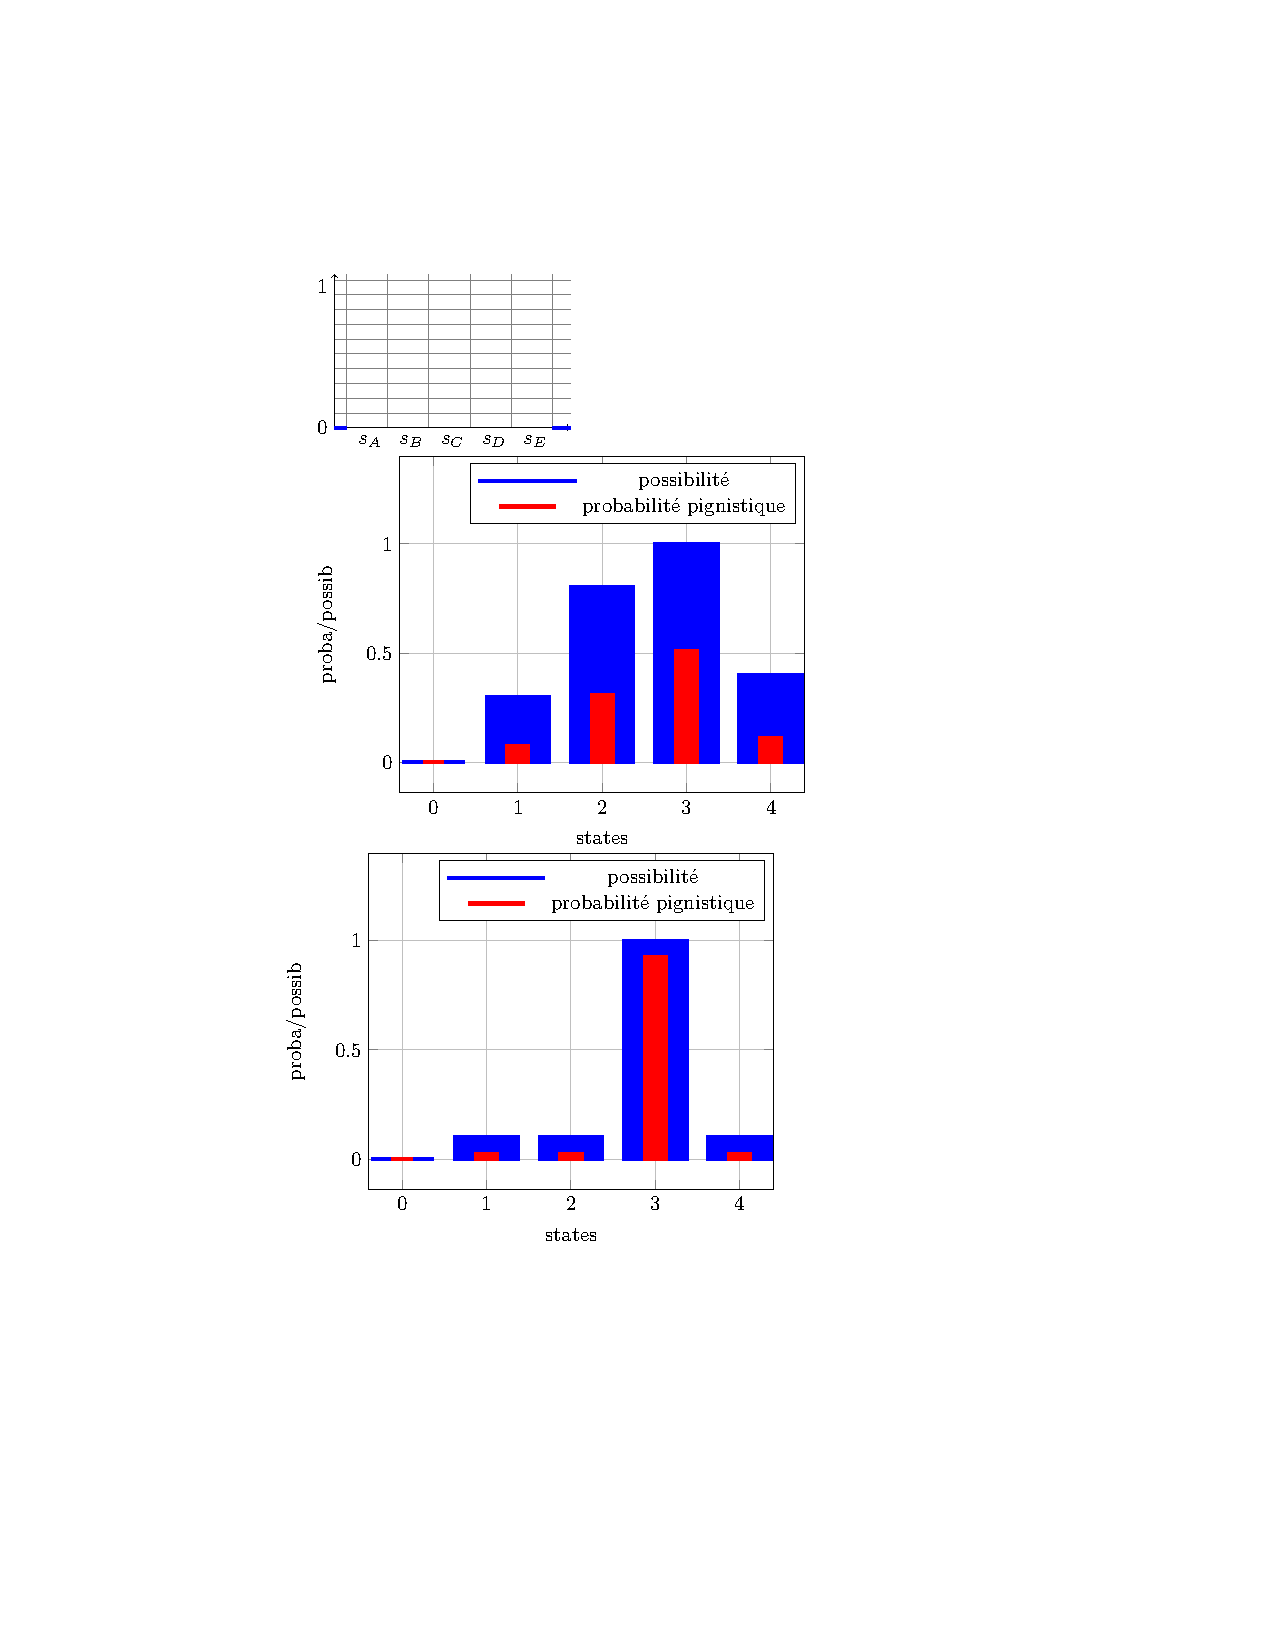
\includegraphics[scale=1.4]{figure.pdf}
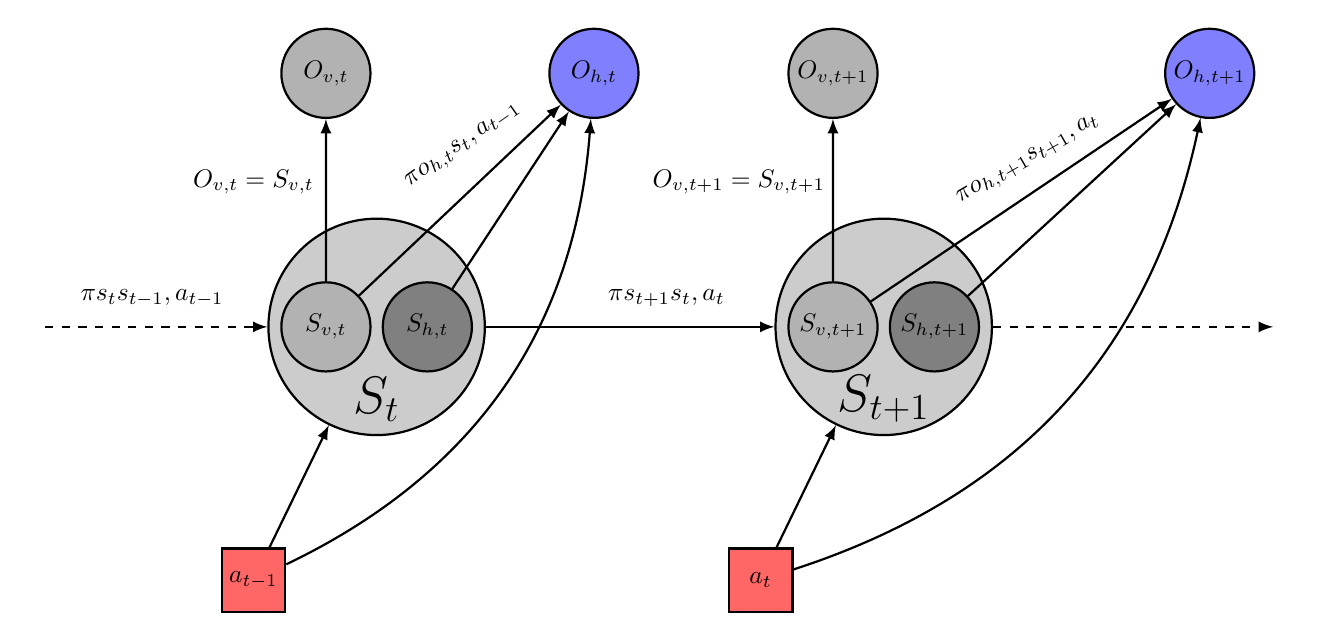
\begin{tikzpicture}[transform shape,scale=0.92]
%% vertex shape and color
\tikzstyle{mvertex}=[circle,fill=black!20,minimum size=85pt,inner sep=0pt,draw=black,thick]
\tikzstyle{vertex}=[circle,fill=black!50,minimum size=35pt,inner sep=0pt,draw=black,thick]
\tikzstyle{vvertex}=[circle,fill=black!30,minimum size=35pt,inner sep=0pt,draw=black,thick]
\tikzstyle{avertex}=[rectangle,fill=red!60,minimum size=25pt,inner sep=0pt,draw=black,thick]
\tikzstyle{rvertex}=[fill=yellow!60,decision=3,inner sep=-1pt,minimum size=35pt,draw=black,thick]
\definecolor{darkgreen}{rgb}{0.3,0.8,0.5}
\tikzstyle{overtex}=[circle,fill=blue!50,minimum size=35pt,inner sep=0pt,draw=black,thick]

%% nodes
% states
\node (G-S_1) at (1.3,0) {};
\foreach \name/\x in {S_t/6, S_{t+1}/13}
\node[mvertex] (G-\name) at (\x,0) {};
\node (G-end) at (18.5,0) {};

\foreach \name/\x in {S_{v,t}/5.3, S_{v,t+1}/12.3}
\node[vvertex] (G-\name) at (\x,0) {$\name$};
\node (vG-end) at (16.5,0) {};

\foreach \name/\x in {S_{h,t}/6.7, S_{h,t+1}/13.7}
\node[vertex] (G-\name) at (\x,0) {$\name$};
\node (hG-end) at (16.5,0) {};


\node (ST) at (6,-1) {\begin{huge}$S_{t}$\end{huge}};
\node (STP1) at (13,-1) {\begin{huge}$S_{t+1}$\end{huge}};

% actions
\foreach \name/\x in {a_{t-1}/2,a_t/9}
\node[avertex] (G-\name) at (\x+2.3,-3.5) {$\name$};

% observations
\foreach \name/\x in {O_{h,t}/6,O_{h,t+1}/14.5}
\node[overtex] (G-\name) at (\x+3,3.5) {$\name$};
% visible ones
\foreach \name/\x in {O_{v,t}/2.3,O_{v,t+1}/9.3}
\node[vvertex] (G-\name) at (\x+3,3.5) {$\name$};

%% arrows
% states
\foreach \from/\to in {S_t/S_{t+1}}
\draw[->,>=latex,thick] (G-\from) -- (G-\to);
\foreach \from/\to in {S_1/S_t,S_{t+1}/end}
\draw[->,>=latex,dashed,thick] (G-\from) -- (G-\to);

% actions
\foreach \from/\to in {a_{t-1}/S_t,a_t/S_{t+1}}
\draw[->,>=latex,thick] (G-\from) -- (G-\to);
\foreach \from/\to in {a_{t-1}/O_{h,t},a_t/O_{h,t+1}}
\draw[->,>=latex,thick] (G-\from) to[bend right]  (G-\to);

% observations
\foreach \from/\to in {S_{h,t}/O_{h,t},S_{h,t+1}/O_{h,t+1}}
\draw[->,>=latex,thick] (G-\from) -- (G-\to);
% from visible states
\foreach \from/\to in {S_{v,t}/O_{h,t},S_{v,t+1}/O_{h,t+1}}
\draw[->,>=latex,thick] (G-\from) -- (G-\to);
% from visible states to visible observations
\foreach \from/\to in {S_{v,t}/O_{v,t},S_{v,t+1}/O_{v,t+1}}
\draw[->,>=latex,thick] (G-\from) -- (G-\to);


\node (pis1) at (2.9,0.4) {$\pi \paren{ s_t \sachant s_{t-1}, a_{t-1}  }$};
\node (pis2) at (10,0.4) {$\pi \paren{ s_{t+1} \sachant s_{t}, a_{t}  }$};
\node (pio1) at (7.2,2.5) [rotate=35] {$\pi \paren{ o_{h,t} \sachant s_t,a_{t-1} }$};
\node (pio2) at (15,2.3) [rotate=30] {$\pi \paren{ o_{h,t+1} \sachant s_{t+1},a_{t} }$};

\node (OVEQUALSV) at (4.3,2) {$O_{v,t} = S_{v,t}$};
\node (OVpEQUALSVP) at (11,2) {$O_{v,t+1} = S_{v,t+1}$};
\end{tikzpicture}
\caption[Dynamic Bayesian Network of a $\pi$-MOMDP]{
Dynamic Bayesian Network of a $\pi$-MOMDP:
at time step $t$, the system state is described 
by variable $S_t = (S_{v,t},S_{h,t})$.
The received observation is $O_t=(O_{v,t},O_{h,t})$
with $O_{v,t}=S_{v,t}$, 
and $O_{h,t}$ depending on $S_t$ and action $a_t$.}
\label{piMOMDP}
\end{figure}

The complexity issue of $\pi$-POMDP solving is due to the fact that the size of the
belief state space $\Pi^{\mathcal{S}}_{\mathcal{L}}$ exponentially grows with the size of the state space $\mathcal{S}$, see the equation (\ref{equation_numberOfPossDistrib})
of Section \ref{section_piPOMDP}.
However, in practice, states are rarely completely hidden.
Using mixed-observability can be a solution: inspired by a similar recent work in probabilistic POMDPs 
\cite{OngShaoHsuWee-IJRR10,AraThoBufCha-ICTAI10}, we present in this section a structured modeling that takes into
account situations where the agent directly observes some part of the state.
a $\pi$-POMDP which models such a situation respects the \textit{mixed-observable property}. 
Belief states are then used only for the partially observed components and the
size of the belief state space is substantially reduced. Thus, this model generalizes both
$\pi$-MDPs and $\pi$-POMDPs.

Like in \cite{AraThoBufCha-ICTAI10}, we assume that the state space $\mathcal{S}$
of a Qualitative Possibilistic Mixed-Observable MDP ($\pi$-MOMDP) 
can be written as a Cartesian 
product of a visible state space $\mathcal{S}_{v}$ and a hidden one $\mathcal{S}_h$: $\mathcal{S}$ = 
$\mathcal{S}_v$ $\times$ $\mathcal{S}_h$.
Let $s=(s_v,s_h)$ be a state of the system. The component $s_v$ is directly
 observed by the agent and $s_h$ is only partially observed through the 
observations of the set $\mathcal{O}_h$: 
we denote by $\pi_t \paren{o_h' \sachant s',a }$,
the possibility distribution over the 
future observation $o_h' \in \mathcal{O}_h$
at time step $t$, 
knowing the future state $s' \in \mathcal{S}$ 
and the current action $a \in \mathcal{A}$. 
Figure \ref{piMOMDP} illustrates the structure 
of this Mixed-Observable model. 

The visible state space is integrated to the observation 
space: $\mathcal{O}_v=\mathcal{S}_v$ and $\mathcal{O}$ = $ \mathcal{O}_v \times \mathcal{O}_h$. Then, knowing
 that the current visible component of the state is $s_v$, the agent
 \textit{necessarily} observes $o_v=s_v$ (if $o_v' \neq s_v$, $\pi_t \paren{ o_v' \sachant s_v } = 0$).
 Formally, seen as a $\pi$-POMDP, its observation possibility 
distribution can be written as:
\begin{eqnarray} 
\nonumber \pi_t \paren{o' \sachant s',a } \hspace{-0.1cm}  & = & \pi_t \paren{ o_v',o_h' \sachant s_v',s_h',a } \\
\nonumber & = & \min \set{ \pi_t \paren{o_h' \sachant s_v',s_h',a }, \pi_t \paren{ o_v' \sachant s_v'} } \\
\label{simplif1}   & = & \left \{ \begin{array}{ccc} 
\pi_t \paren{ o_h' \sachant s',a } & \mbox{if  } o_v' = s_v' \\
0 & \mbox{otherwise} 
\end{array} \right.
\end{eqnarray}
since $\pi_t \paren{ o_v' \sachant s_v'} = 1$ if $s_v'=o_v'$ and $0$ otherwise. 
The following theorem, based on this equality enables the
belief over hidden states to be defined.
\begin{theorem}[Nature of Reachable Belief States]
\label{thm_natureReachBel} Each reachable belief state of a $\pi$-MOMDP can be
written as an element of $\mathcal{S}_v \times \Pi^{\mathcal{S}_h}_{\mathcal{L}}$ where $\Pi^{\mathcal{S}_h}_{\mathcal{L}}$
is the set of possibility distributions over $\mathcal{S}_h$: any $\beta \in \Pi^{\mathcal{S}_h}_{\mathcal{L}}$
can be written as $(s_v,\beta_h)$ with $\beta_h(s_h) = \max_{\overline{s}_v \in \mathcal{S}_v} \beta(\overline{s}_v,s_h)$ and $s_v = \operatorname*{argmax}_{\overline{s}_v \in \mathcal{S}_v} \beta(\overline{s}_v,s_h)$.
\end{theorem}
The proof is given in Annex \ref{thm_natureReachBel_RETURN}

As all reachable belief states are in $\mathcal{S}_v \times \Pi^{\mathcal{S}_h}_{\mathcal{L}}$
when the mixed-observability property holds, 
the next theorem rewrites the belief update function for the belief states 
$\beta_h \in \Pi^{\mathcal{S}}_{\mathcal{L}}$ over the hidden system states $s_h \in \mathcal{S}_h$.
\begin{theorem}[Belief Update for a $\pi$-MOMDP]
\label{thmMomdpBelup}
If a problem can be modeled by a $\pi$-MOMDP  
\[ \Big\langle S_v \times S_h, \mathcal{A}, \mathcal{O}_h, T^{\pi}, O^{\pi}, (\rho_t)_{t=0}^{H-1}, \Psi, \beta_0 = (s_{v,0}, \beta_{h,0})  \Big\rangle, \]
a new belief update function $\nu_h$ can be defined:
if, at time step $t$, 
the current visible state is $s_{v,t} \in \mathcal{S}_v$,
the current belief state about the hidden system state is $\beta_{h,t} \in \Pi^{\mathcal{S}_h}_{\mathcal{L}}$,
the selected action is $a_t \in \mathcal{A}$,
the next visible state is $s_{v,t+1} \in \mathcal{S}_v$
and the next observation is $o_{h,t+1} \in \mathcal{O}_h$,
then the next belief state about the hidden system state is
\begin{equation}
\label{equation_piMOMDPupdate}
\beta_{h,t+1}(s_h') = \left \{ \begin{array}{ccc}
1 & \mbox{ if } \left. \begin{array}{cc} \pi_t \paren{ s_h', s_{v,t+1}, o_{h,t+1} \sachant s_{v,t}, \beta_{h,t}, a_t } \\
	 	= \pi_t \paren{s_{v,t+1}, o_{h,t+1} \sachant s_{v,t}, \beta_{h,t}, a_t }
		\end{array} \right., \\
\\
\pi_t \paren{ s_h', s_{v,t+1}, o_{h,t+1} \sachant s_{v,t}, \beta_{h,t}, a_t } & \mbox{ otherwise } 
\end{array} \right. 
\end{equation}
where 
\[ \pi_t \paren{s_v',  s_h', o_h' \sachant s_v, \beta_h, a } = \min \Big\{ \pi_t \paren{ o_h' \sachant s', a  }, \max_{s_h \in \mathcal{S}_h} \min \set{ \pi_t \paren{s' \sachant s_v,s_h, a}, \beta_h(s_h)  } \Big\} \] 
is the joint possibility distribution over hidden system states $s_h' \in \mathcal{S}_h$ 
and visible objects (visible system state and observation) $s_v' \in \mathcal{S}_v$ and $o_h' \in \mathcal{O}_h$.
The notation $\pi_t \paren{ s_v', o_h' \sachant s_v, \beta_h, a }$ 
is for the possibility degree of the visible objects
$\max_{s_h' \in \mathcal{S}_h} \pi_t \paren{ s_h', s_v', o_h' \sachant s_v, \beta_h, a }$
(using the notation $s' = (s_v', s_h') \in \mathcal{S} = \mathcal{S}_v \times \mathcal{S}_h$). 
This belief update is denoted by \[ \beta_h' = \nu_h \paren{ s_v, \beta_h, a, s_v', o_h' }. \]
\end{theorem}
The proof is given in Annex \ref{thmMomdpBelup_RETURN}.

The state space of the belief $\pi$-MDP resulting from a $\pi$-MOMDP 
can be restricted to the product space $\mathcal{S}_v \times \Pi^{\mathcal{S}_h}_{\mathcal{L}}$,
\textit{i.e.} 
a finer belief $\pi$-MDP than those presented previously, 
benefiting from the Mixed-Observability,
can be defined: 
$\langle \tilde{S}^{\pi}, \tilde{T^{\pi}}, \mathcal{A}, (\tilde{\rho_t})_{t=0}^{H-1}, \tilde{\Psi} \rangle$,
where
\begin{itemize}
\item the state space of the belief $\pi$-MDP is defined as $\tilde{S}^{\pi} = \mathcal{S}_v \times \Pi^{\mathcal{S}_h}_{\mathcal{L}}$,
\item a transition possibility distribution in $\tilde{T^{\pi}}$ is such that $\forall \set{ 0, \ldots, H-1 }$, $\forall a \in \mathcal{A}$,
$\forall \Big[ (s_v,\beta_h), (s_v',\beta_h') \Big]  \in \Big(\tilde{S}^{\pi}\Big)^2$, 
\[ \pi_t \Big( (s_v',\beta_h') \Big\vert (s_v,\beta_h), a  \Big) = \max_{\substack{ o_h' \in \mathcal{O}_h \mbox{ \tiny s.t. } \\ \nu_h(s_v,\beta_h,a,s_v',o_h') = \beta_h'}}
\pi_t \paren{ s_v',o_h' \sachant s_v, \beta_h, a },  \]
where $\pi_t \paren{ s_v',o_h' \sachant s_v, \beta_h, a }$ is defined just above,

\item If the belief-based preferences are optimistic \textit{i.e.}
$\tilde{\rho_t}=\overline{\rho_t}$ and $\tilde{\Psi}=\overline{\Psi}$,
then $\forall t \in \set{ 0, \ldots, H-1 }$, $\forall s_v \in \mathcal{S}_v$,
$\forall \beta_h \in \Pi^{\mathcal{S}_h}_{\mathcal{L}}$, $\forall a \in \mathcal{A}$,  
the preference functions can be rewritten
\[ \overline{\rho_t}(s_v,\beta_h) = \max_{s_h \in \mathcal{S}_h} \min \set{ \rho_t(s_v,s_h), \beta_h(s_h) }, \]
and
\[ \overline{\Psi}(s_v,\beta_h) = \max_{s_h \in \mathcal{S}_h} \min \set{ \Psi(s_v,s_h), \beta_h(s_h) }. \]
Indeed, $\beta(\overline{s_v},s_h) = 0$ 
if $\overline{s_v}$ is not the 
actual visible state $s_v$, 
thus, for instance
\begin{eqnarray*}
\overline{\Psi}(\beta) & = & \max_{s \in \mathcal{S}} \min \set{ \Psi(s), \beta(s)} \\
 & = & \max_{s_h \in \mathcal{S}_h} \min \set{ \Psi(s_v,s_h), \beta(s_h,s_v)}.
\end{eqnarray*} 
\item If the belief-based preferences are pessimistic \textit{i.e.}
$\tilde{\rho_t}=\underline{\rho_t}$ and $\tilde{\Psi}=\underline{\Psi}$,
then $\forall t \in \set{ 0, \ldots, H-1 }$, $\forall s_v \in \mathcal{S}_v$,
$\forall \beta_h \in \Pi^{\mathcal{S}_h}_{\mathcal{L}}$, $\forall a \in \mathcal{A}$,  
the preference functions can be rewritten
\[ \underline{\rho_t}(s_v,\beta_h) = \min_{s_h \in \mathcal{S}_h} \max \set{ \rho_t(s_v,s_h), 1 - \beta_h(s_h) }, \]
and
\[ \underline{\Psi}(s_v,\beta_h) = \min_{s_h \in \mathcal{S}_h} \max \set{ \Psi(s_v,s_h), 1 - \beta_h(s_h) }. \]
Indeed, $1 - \beta(\overline{s_v},s_h) = 1$ 
if $\overline{s_v}$ is not the 
actual visible state $s_v$, 
thus, for instance
\begin{eqnarray*}
\underline{\Psi}(\beta) & = & \min_{s \in \mathcal{S}} \max \set{ \Psi(s), 1 - \beta(s)} \\
 & = & \min_{s_h \in \mathcal{S}_h} \max \set{ \Psi(s_v,s_h), 1 - \beta(s_h,s_v)}.
\end{eqnarray*} 
\end{itemize}

\vbox{
\begin{theorem}[Dynamic Programming Equation of a $\pi$-MOMDP]
\label{theorem_DPpiMOMDP}
The dynamic programming equation becomes:\\ 
$\forall (s_v,\beta_h) \in \mathcal{S}_v \times \Pi^{\mathcal{S}_h}_{\mathcal{L}}$,
\[ \widehat{U_{0}^*}(s_v,\beta_h) = \tilde{\Psi}(s_v,\beta_h), \]
and, $\forall i \in \{1,\ldots,H \}$, $\forall (s_v,\beta_h) \in \mathcal{S}_v \times \Pi^{\mathcal{S}_h}_{\mathcal{L}}$,  
\[ \widehat{U}^*_i(s_v,\beta_h)  = \max_{a \in \mathcal{A}} \widehat{M} \Bigg\{ \tilde{\rho_t}(s_v,\beta_h,a), \widehat{\mathbb{S}}\bigg( \pi_t \paren{s_v',o_h' \sachant s_v, \beta_h, a}, \widehat{U^*_{i-1}} \Big( \nu_h( s_v,\beta_h,a,s_v',o_h') \Big) \bigg)  \Bigg\}, \]
\begin{equation}
\label{equation_MOactionselection}
\widehat{\delta}^*_i(s_v,\beta_h) \in \operatorname*{argmax}_{a \in \mathcal{A}} \widehat{M} \Bigg\{ \tilde{\rho_t}(s_v,\beta_h,a), \widehat{\mathbb{S}}\bigg( \pi_t \paren{s_v',o_h' \sachant s_v, \beta_h, a}, \widehat{U^*_{i-1}} \Big( \nu_h( s_v,\beta_h,a,s_v',o_h') \Big) \bigg)  \Bigg\},
\end{equation}
where $\nu_h$ is the new belief update function (Theorem \ref{thmMomdpBelup}), 
and the notations come from the general Dynamic Programming Equation \ref{general_DP_piPOMDP}.
%%
%%
%%\max_{s_v' \in S_v} \max_{o_h' \in O_h} \min \set{ \beta^a(s_v',o_h'), \overline{U}_{i-1}^*(s_v',\nu_h(\beta_h^{a,s_v',o_h'}))	 }
%%\]
%with the initialization \hspace{0.5cm} $u^*_0(s_v,\beta_h) = \mu(s_v,\beta_h) $,
%where $ \mu(s_v,\beta_h) = \displaystyle \min_{s_h \in \mathcal{S}_h} \max \set{ \mu(s_v,s_h), n( \beta_h(s_h) ) }$
%\\
%is the preference over $S_v \times B^{\pi}_h$, \\ 
%\begin{equation*}
%\beta^a(s_v',o_h') = \displaystyle \max_{s_h' \in \mathcal{S}_h} \min \set{\pi \paren{ o_h' \sachant s_v',s_h',a }, \beta^a(s_v',s_h') },
%\end{equation*}
%
\end{theorem}
The proof is given in Annex \ref{theorem_DPpiMOMDP_RETURN}.
}

A standard algorithm would have computed $\widehat{U_i^*}(\beta)$ for each
 $\beta \in \Pi^{\mathcal{S}}_{\mathcal{L}}$ 
while this new dynamic programming equation 
leads to an algorithm 
which computes it only 
for all $(s_v,\beta_h) \in \mathcal{S}_v \times 
\Pi^{\mathcal{S}_h}_{\mathcal{L}}$,
since only this kind of belief states can be encountered. 
The size of the new belief space is 
\[ \# (\mathcal{S}_v \times \Pi^{\mathcal{S}_h}_{\mathcal{L}})
= \# \mathcal{S}_v \times \paren{ \# \mathcal{L}^{\# \mathcal{S}_h} - (\# \mathcal{L}-1)^{\# \mathcal{S}_h} }, \] 
which is exponentially smaller than the size of standard 
$\pi$-POMDPs' belief space: 
\[ \# \Pi^{\mathcal{S}}_{\mathcal{L}} = \# \mathcal{L}^{\# \mathcal{S}_v \times \# \mathcal{S}_h} - (\# \mathcal{L}-1)^{\# \mathcal{S}_v \times \# \mathcal{S}_h}. \]
An even finer belief $\pi$-MDP 
could be defined on the set of reachable belief states 
starting from the initial belief state $\beta_0$: 
$\Pi^{\mathcal{S}}_{\mathcal{L},\beta_0}$ which is a subset of 
$\Pi^{\mathcal{S}_h}_{\mathcal{L}}$. 

\section{Infinite Horizon Settings}
\label{section_infiniteHorizon}
A finite strategy for possibilistic MOMDPs can now be computed for
larger problems using the dynamic programming equation of Theorem \ref{theorem_DPpiMOMDP} 
and selecting maximizing actions for each state $(s_v,\beta_h) \in \mathcal{S}_v \times \Pi^{\mathcal{S}_h}_{\mathcal{L}}$
(see the equation \ref{equation_MOactionselection}), 
as done in the equation (\ref{general_DP_piPOMDP_actSelec}) 
for each $\beta \in \Pi^{\mathcal{S}}_{\mathcal{L}}$.
%Algorithm \ref{piMDP_horizon_fini}.
However, for many problems in practice, 
it is difficult to determine a horizon size $H$. 
The goal of this section is to present
an algorithm to solve optimistic $\pi$-MOMDPs with terminal preference only,
under infinite horizon:
it is the first proved algorithm to solve such $\pi$-(MO)MDPs.
%For this purpose, we first propose a Value Iteration algorithm for $\pi$-MDPs whose optimality of the returned policy is shown in Appendix \ref{proofThmIV}.
%Then the $\pi$-MOMDPs one is given and the optimality is provided
%using the previous result.

\subsection{The $\pi$-MDP case}
\label{subsection_piVI}
Previous work, \cite{Sabbadin:1999:pipomdp,Sabbadin2001287}, 
on solving $\pi$-MDPs proposed a Value Iteration
algorithm that was proved to compute optimal value functions, but not
necessarily optimal strategies for some problems with cycles. 
There is a similar issue 
in \emph{undiscounted} probabilistic MDPs 
where the greedy strategy at convergence of Value Iteration 
does not need to be optimal \cite{puterman94}.
It is not surprising that we are facing the same issue in $\pi$-MDPs since the
possibilistic dynamic programming operator does not rely on algebraic products
so that it cannot be contracted by some \textit{discount factor} $0 < \gamma < 1$.

For infinite horizon problems, the optimistic $\pi$-MDP model 
has to undergo a little change.
The dynamics is defined as stationary,
as in the probabilistic case, see Section \ref{subsectionIHMDP}:
$\forall t \geqslant 0$,
$\forall (s,s') \in \mathcal{S}^2$, $\forall \in \mathcal{A}$,
\[ \pi_t \paren{ s' \sachant s,a  } = \pi \paren{ s' \sachant s,a  }. \]
The case of terminal preference only, is considered: 
starting from the general optimistic $\pi$-MDP 
(with intermediate preferences and minimum-based global preference,
see Section \ref{subsection_piMDPs}) 
the preference functions can be set equivalently to 
$\forall t \geqslant 0$, $\forall s \in \mathcal{S}$, $\forall \in \mathcal{A}$,
\[ \rho_t(s,a) = 1,\]
and thus, only the terminal preference function $\Psi$
has an effect on the criterion,
and has to be defined 
for the instantiation of the $\pi$-MDP.

\begin{algorithm} \caption{ Optimistic $\pi$-MDP VI Algorithm -- Terminal Preference Only} 
\label{algorithmIVPIMDP}
\For {$s \in \mathcal{S}$}{
	$\overline{U^*}(s) \gets 0$ \;
	$\overline{U^c}(s) \gets \Psi(s)$ \;
	$\overline{\delta^*}(s) \gets \widehat{a}$ \;
}
\While {$\overline{U^*} \neq \overline{U^c}$ }{
\label{beginning_while_VI}	$\overline{U^*}=\overline{U^c}$ \;
	\For {$s \in \mathcal{S}$}{
		$\displaystyle \overline{U^c}(s) \gets \max_{a \in \mathcal{A}} \max_{s' \in \mathcal{S}} \min \set{ \pi \paren{ s' \sachant s,a }, \overline{U^*}(s') }$ \label{VIupdate_OptAlgo} \;
		\If {$\overline{U^c}(s)>\overline{U^*}(s)$}{
			$ \displaystyle \overline{\delta^*}(s) \in \operatorname*{argmax}_{a \in \mathcal{A}} \max_{s' \in \mathcal{S}} \min \set{ \pi \paren{ s' \sachant s,a }, \overline{U^*}(s') }$ \;
 		}
 	}
}
\Return $\overline{U^*}$, $\overline{\delta^*}$ \;
\end{algorithm}

To the best of our knowledge, we propose here the first Value Iteration algorithm 
 for $\pi$-MDPs, 
that provably returns an optimal strategy, and that is different
from the one of \cite{Sabbadin2001287}. Indeed, in the deterministic example of Figure \ref{figExample},
 action $\widehat{a}$, which is clearly suboptimal in state $s_A$, 
was found to be optimal in $s_A$ with this algorithm: 
however it is clear that since 
$\pi \paren{ s_B \sachant s_A, b} = 1$ and $\Psi(s_B)=1$, $\overline{U^*_1}(s_A) = 1$.
 Obviously, $\overline{U^*_1}(s_B) = 1$ and since
$\pi \paren{ s_A \sachant s_A, \widehat{a} } = 1$,
$\max_{s' \in \mathcal{S}} \min \set{ \pi  \paren{ s' \sachant s_A,a }, \overline{U^*_1}(s') } 
= 1$ $\forall a \in \set{ \widehat{a}, b } = \mathcal{A}$, 
\textit{i.e.} all actions are optimal in $s_A$. 
The ``if'' condition of Algorithm \ref{algorithmIVPIMDP} 
permits to select the optimal action $b$ during the first step. 
This condition and the initialization, 
which were not present in previous algorithms of the literature, 
are needed to prove the optimality of the strategy.
\begin{figure} \caption{Deterministic example showing the limits of previous algorithms}\centering
\begin{tikzpicture}[scale=1.5] \label{figExample} 
\tikzstyle{mvertex}=[circle,fill=black!15,minimum size=20pt,inner sep=0pt]
\node (origine) at (2.6,0) {};
\node[mvertex] (state1) at (4,0) {$s_A$};
\node[mvertex] (state2) at (8,0) {$s_B$};
\draw[->,>=latex] (state1) to[bend left] (state2);
\node (rester) at (2.7,0) {$\widehat{a}$};
\node (bouger) at (6,0.2) {$b$};
\node (actions2) at (9.2,0) {$\widehat{a},b$};
\node (rec1) at (5,-0.5) {$\Psi(s_A)=0$};
\node (rec2) at (8.9,0.7) {$\Psi(s_B)=1$};
%\draw[->,>=latex] (state1) to[bend left] (state1);
\draw[->,>=latex] (state1)..controls +(-1,1) and +(-1,-1).. (state1);
\draw[->,>=latex] (state2)..controls +(1,1) and +(1,-1).. (state2);
%\draw (state1.north west) to[bend right] (state1.south west);
\end {tikzpicture}
\end{figure}
The proof, which is quite lengthy and intricate, 
is presented in Annex \ref{proofThmIV}. 
This sound algorithm for $\pi$-MDPs 
will then be extended to $\pi$-MOMDPs in the next section.

As mentioned in \cite{Sabbadin:1999:pipomdp}, 
we assume the existence of an action ``stay'', 
denoted by $\widehat{a}$, 
which lets the system in the same state with necessity $1$. 
This action is the possibilistic counterpart 
of the discount parameter $\gamma$ in the probabilistic model, 
as it guarantees convergence of the Value Iteration algorithm. 
However, we will see that action $\widehat{a}$ 
is finally used only on some particular satisfactory states. 
Note that a similar assumption is used to compute optimal strategies
in the framework of deterministic processes (classical planning)
whose horizon is not specified \cite{LaValle2006PA1213331}.

We denote by $\widehat{\delta}$ the decision rule 
such that $\forall s \in \mathcal{S}$, $\widehat{\delta}(s)=\widehat{a}$. 
The set of all the finite strategies is 
$\Delta =\cup_{i \geqslant 1} \Delta_i$, 
and $\# \delta$ is the size of a strategy $(\delta)$ 
in terms of decision epochs. 
We can now define the optimistic criterion 
for an infinite horizon: 
if $(\delta) \in \Delta$,
\begin{equation} 
\label{optcriterion} 
\overline{U} \Big( s_0,(\delta) \Big) 
= \max_{ \mathcal{T} \in \mathcal{T}_{\# \delta}} 
\min \bigg\{ \pi \Big( \mathcal{T} \Big\vert s_0, (\delta) \Big), \Psi(s_{\# \delta}) \bigg\},
\end{equation}
where $\mathcal{T} = (s_1,\ldots,s_{\# \delta})$ is a trajectory of system states,
$\mathcal{T}_{\# \delta}$ the set of such trajectories,
and 
\[ \pi \Big( \mathcal{T} \Big\vert s_0, (\delta) \Big) 
= \min_{i=0}^{\# \delta - 1} \pi \Big( s_{i+1} \Big\vert s_i, \delta_i(s_i)  \Big). \]
\begin{theorem}[Optimality of the VI Algorithm for Optimistic $\pi$-MDPs]
\label{thmIV} If there exists an action $\widehat{a}$ such that, 
for each $s \in \mathcal{S}$, $\pi \paren{s' \sachant s, \widehat{a} } = 1$ 
if $s'=s$ and $0$ otherwise, 
then Algorithm \ref{algorithmIVPIMDP} 
computes the maximum optimistic criterion 
and an optimal strategy,
\textit{i.e.} maximizing the criterion (\ref{optcriterion}),
which is stationary 
(\textit{i.e.} which does not depend on the stage of the process $t$).
\end{theorem}
The proof is given in Annex \ref{proofThmIV}. Note that, as in the probabilistic case
(see Section \ref{resMDP}), the computed optimal strategy is stationary
\textit{i.e.} does not depend on the time step of the process.

Let $s$ be a state such that $\overline{\delta^*}(s)=\widehat{a}$, 
where $\overline{\delta^*}$ is the returned strategy. 
By looking at Algorithm \ref{algorithmIVPIMDP}, 
it can be noted that $\overline{U^*}(s)$ 
always remains equal to $\Psi(s)$ 
during the iterations of the algorithm
after the first entry in the while loop.
Thus, $\forall s' \in \mathcal{S}$, 
either $\forall a \in \mathcal{A}$, 
$\Psi(s) \geqslant \pi \paren{s' \sachant s,a}$, 
or $\Psi(s) \geqslant \overline{U^*}(s')$. 
If the problem is non trivial, 
it means that $s$ is a goal ($\Psi(s)>0$) 
and that degrees of possibility of transitions to better goals 
are less than the degree of preference for $s$.

\subsection{Value Iteration for $\pi$-MOMDPs}
\label{section_VIpiMOMDP}
We are now ready to propose the Value Iteration algorithm for $\pi$-MOMDPs
which reduces to a belief $\pi$-MDP which is optimistic and with terminal preference only
(whose Value Iteration algorithm has been presented in the previous section).
This Value Iteration algorithm is, for instance, devoted to $\pi$-MOMDPs 
with the $\pi$-POMDP mixed optimistic-pessimistic criterion,
see Definition \ref{def_optpesscrit}: the terminal preference function is then
$\underline{\Psi}(s_v,\beta_h) = \min_{s_h \in \mathcal{S}_h} \max \set{ \Psi(s_v,s_h) , 1 - \beta_h(s_h) }$.
Another example of appropriate $\pi$-MOMDP 
with the optimistic $\pi$-POMDP criterion 
(see Algorithm \ref{PIPOMDP_algo_opt_intermpref}, removing intermediate preferences):
the terminal preference function is in this case
$\overline{\Psi}(s_v,\beta_h) = \max_{s_h \in \mathcal{S}_h} \min \set{ \Psi(s_v,s_h) ,\beta_h(s_h) }$.

\begin{algorithm} \caption{ $\pi$-MOMDP Value Iteration Algorithm} \label{algorithmpiMOMDP}
\SetKw{KwAnd}{and}
\For {$s_v \in \mathcal{S}_v$ \KwAnd $\beta_h \in \Pi^{\mathcal{S}_h}_{\mathcal{L}}$}{
 	$\overline{U^*}(s_v,\beta_h) \gets 0$ \;
 	$\overline{U^c}(s_v,\beta_h) \gets \tilde{\Psi}(s_v,\beta_h)$ \;
 	$\overline{\delta^*}(s_v,\beta_h) \gets \widehat{a}$ \;
}
\While {$\overline{U^*} \neq \overline{U^c}$ }{
 	$\overline{U^*} \gets \overline{U^c}$ \;
 	\For {$s_v \in \mathcal{S}_v$ \KwAnd $\beta_h \in \Pi^{\mathcal{S}_h}_{\mathcal{L}}$}{
 		$\displaystyle \overline{U^c}(s_v,\beta_h) \gets \max_{a \in \mathcal{A}} \max_{s_v' \in \mathcal{S}} \max_{o_h' \in \mathcal{O}_h} \min \bigg\{ \pi \Big( s_v', o_h' \Big\vert s_v, \beta_h, a \Big), \overline{U^*}\Big(s_v',\nu_h(s_v,\beta_h,s_v',o_h') \Big) \bigg\}$ \label{piMOMDP_VIupdate}  \;
 		\If {$\overline{U^c}(s_v,\beta_h)>\overline{U^*}(s_v,\beta_h)$}{
 			\mbox{$\displaystyle \overline{\delta^*}(s_v,\beta_h) \in \operatorname*{argmax}_{a \in \mathcal{A}} \max_{s_v' \in \mathcal{S}} \max_{o_h' \in \mathcal{O}_h} \min \bigg\{ \pi \Big( s_v', o_h' \Big\vert s_v, \beta_h, a \Big), \overline{U^*}\Big(s_v',\nu_h(s_v,\beta_h,s_v',o_h') \Big) \bigg\}$ \;}
 		}
 	}
}
\Return $u^*$, $\delta^*$ \;
\end{algorithm}
Note that Algorithm \ref{algorithmpiMOMDP} has the same structure 
as Algorithm \ref{algorithmIVPIMDP}. 
Note as well that a $\pi$-MOMDP is a $\pi$-MDP 
over $\mathcal{S}_v \times \Pi^{\mathcal{S}_h}_{\mathcal{L}}$. 
Recall that the transition possibility distribution is
\[ \pi_t \Big( (s_v',\beta_h') \Big\vert (s_v,\beta_h), a  \Big) = \max_{\substack{ o_h' \in \mathcal{O}_h \mbox{ \tiny s.t. } \\ \nu_h(s_v,\beta_h,a,s_v',o_h') = \beta_h'}}
\pi_t \paren{ s_v',o_h' \sachant s_v, \beta_h, a }. \]
%Let $s_v \in \mathcal{S}_v$, $\beta_h \in \Pi^{\mathcal{S}_h}_{\mathcal{L}}$ 
%and now $\mathcal{O}_h^{s_v,\beta_h,\widehat{a},s_v'}(\beta_h')
%=\set{ o_h' \in \mathcal{O}_h \sachant \nu_h(s_v,\beta_h,\widehat{a},s_v',o_h')= \beta_h' }$. 
To satisfy the assumption of Theorem \ref{thmIV}, 
it suffices to ensure that 
$\pi_t \Big( (s_v',\beta_h') \Big\vert (s_v,\beta_h), a  \Big) = 1$
if $s_v'=s_v$ and $\beta_h'=\beta_h$,
and $0$ otherwise.
%$\max_{o_h' \in \Gamma_{\beta,\widehat{a},s_v'}(\beta_h')}\beta^{\widehat{a}}(s_v',o_h')=1$ 
%if $s_v'=s_v$ and $\beta_h'=\beta_h$ and $0_\mathcal{L}$ otherwise. 
This property is verified if the two following conditions hold: 
$\pi \paren{ s_v',s_h' \sachant s_v,s_h, \widehat{a} } = 1$ 
if $(s_v',s_h')=(s_v,s_h)$, and $0$ otherwise, 
and there exists an observation ``nothing'' $\widehat{o_h}$ 
that is required for each state when $\widehat{a}$ is chosen
\textit{i.e.} 
$\forall (s_v',s_h') \in \mathcal{S}$,
$\pi \paren{ o_h' \sachant s_v',s_h',\widehat{a}} = 1$ if $o_h'=\widehat{o_h}$ and $0$ otherwise.
Indeed, it means that $\widehat{o_h}$ is received for sure when $\widehat{a}$ is selected:
no information is provided by this observation,
and the belief does not evolve. 

\section{Results on a Robotic Mission and Possibilistic Belief State Behaviour}
\label{EXPE_CHAP1}
This section is devoted to the use of strategies computed 
by Algorithm \ref{algorithmpiMOMDP} 
in the context of a concrete robotic problem. 
Consider a robot over a grid of size $g \times g$, with $g>1$. 
It always perfectly knows its location on the grid $(x,y) \in \{ 1, \ldots, g \}^2$, 
which forms the visible state space $\mathcal{S}_v$. 
It starts at location $s_{v,0}=(1,1)$.
Two targets are located at $(x_1,y_1)=(1,g)$ (``target $1$'') 
and $(x_2,y_2)=(g,1)$ (``target $2$'') on the grid, 
and the robot perfectly knows their positions. 
One of the targets is $A$, the other $B$ 
and the robot's mission is to identify and reach target $A$ 
as soon as possible. 
The robot does not know which target is $A$: 
the two situations, ``target $1$ is $A$'' ($A1$) 
and ``target $2$ is $A$'' ($A2$), 
constitute the hidden state space $\mathcal{S}_h$. 
The moves of the robot are deterministic 
and its actions $\mathcal{A}$ 
consist in moving in the four directions plus the action ``stay''.
At each stage of the process, 
the robot analyzes pictures of each target 
and gets then an observation of the targets' natures: 
the two targets ($oAA$) can be observed as A, 
or target $1$ ($oAB$), or target $2$ ($oBA$) or no target ($oBB$).

In the probabilistic framework, 
the probability of having a good observation of target $i \in \{ 1,2 \}$, 
is not really known but approximated by 
$\textbf{p} \paren{ good_i \sachant x,y } 
= \frac{1}{2} \croch{ 1 + \exp \paren{ -\frac{\sqrt{(x-x_i)^2+(y-y_i)^2}}{D} } }$ 
where $(x,y)$ $=s_v$ $\in \{ 1,\ldots,g \}^2 $
is the location of the robot, 
$(x_i,y_i)$ the position of target $i$, 
and $D$ a normalization constant. 
We suppose that the observations 
of both targets are independent:
then, for instance, the probability 
$\textbf{p} \paren{ oAB \sachant (x,y), A1 }$ is equal to 
$\textbf{p} \paren{ good_1 \sachant (x,y)} 
\cdot \textbf{p} \paren{ good_2 \sachant (x,y) }$, 
$\textbf{p} \paren{ oAA \sachant (x,y), A1 }$ 
to $\textbf{p}\paren{ good_1 \sachant (x,y)} 
\cdot \croch{ 1 - \textbf{p} \paren{ good_2 \sachant (x,y) } } $, 
and so on. 
Each step of the process before reaching a target costs $1$, 
reaching target $A$ is rewarded by 100, 
and -100 for $B$. 
The probabilistic strategy was computed 
in mixed-observability settings with APPL\footnote{The used software is available at \url{http://bigbird.comp.nus.edu.sg/pmwiki/farm/appl/}} 
based on SARSOP \cite{OngShaoHsuWee-IJRR10,Kurniawati-RSS08}
(see Section \ref{section_SAalgo}), 
using a precision of $0.046$ 
(the memory limit is reached for higher precisions) 
and a discount factor $\gamma=0.99$. 
This problem cannot be solved 
with the exact algorithm for MOMDPs \cite{AraThoBufCha-ICTAI10} 
because it consumes the entire RAM after $15$ iterations.

In the framework of Qualitative Possibility Theory, 
it is considered always possible to observe the good target: 
$\pi \paren{good \sachant x,y}=1$. 
Secondly, the farther the robot is from target $i$, 
the more likely it is to badly observe it 
(e.g. observe $A$ instead of $B$), 
which is a reasonable assumption 
if the actual probabilistic observation model is
imprecisely known: 
$\pi \paren{ bad_i \sachant x,y } 
= \frac{(x-x_i)^2 + (y-y_i)^2 }{2(g-1)^2}$,
and thus, $\mathcal{L}$
can be defined by $\set{ 0, \frac{1}{2(g-1)}, \ldots, 1}$,
or any other scale preserving the fact
that the possibility degree of misperceiving 
increases with the distance from the considered target. 
The observation of a target is also considered 
as NI-independent from the the observation of the other target
(see Definition \ref{def_NIindep} of Section \ref{qualitative_indep}).
Thus for instance, 
$\pi \paren{ oAB \sachant (x,y), A1 }=1$, 
$\pi \paren{ oAA \sachant (x,y), A1 } 
= \pi \paren{ bad_2 \sachant x,y } $, 
$\pi \paren{ oBA \sachant (x,y), A1 } 
= \min \set{ \pi \paren{ bad_1 \sachant x,y },
\pi \paren{ bad_2 \sachant \hspace{-0.1cm} x,y }} $, etc.
%Note that the situation is fully known 
%when the robot is at a target's location: 
%thus there is no risk of being blocked 
%in an unsatisfactory state, 
%that is why using the \textit{optimistic} 
%$\pi$-MOMDP works quite well.
%$\mathcal{L}$ thus consists in $0$, $1$, 
%and all the other intermediate possible values of 
%$\pi \paren{ bad \sachant x,y }$. 
Note that the construction of this model 
with a probability-possibility transformation 
\cite{Dubois93onpossibility/probability} 
would have been equivalent. 
The terminal preference function $\Psi$ is equal to $0$ 
for all the system's states
and to $1$ for states 
$[(x_{1},y_{1}),A1]$ and $[(x_{2},y_{2}),A2]$ 
where $(x_{i},y_{i})$ is the position of target $i$. 
As mentioned in \cite{Sabbadin:1999:pipomdp}, 
the computed strategy guarantees a shortest path to a goal state.
The strategy then aims at reducing the mission duration.
The mixed optimistic-pessimistic criterion,
see Definition \ref{def_optpesscrit},
is used here to compute the strategy.


Standard $\pi$-POMDPs, which do not exploit mixed-observability 
contrary to our $\pi$-MOMDP model, 
could not solve even very small $3 \times 3$ grids.
Indeed, for this problem, 
$\# \mathcal{L} \geqslant 5$, 
$\# \mathcal{S}_v = 9 $, 
and $\# \mathcal{S}_h = 2$. 
Thus, $\# \mathcal{S} = \# \mathcal{S}_v \times \# \mathcal{S}_h = 18$ 
and the number of belief states is then 
$\# \Pi^{\mathcal{S}}_{\mathcal{L}} 
= \mathcal{L}^{\# \mathcal{S}} - (\mathcal{L}-1)^{\# \mathcal{S}} 
\geqslant 5^{18} -4^{18} 
\geqslant 3.7.10^{12}$ 
instead of $81$ states with a $\pi$-MOMDP. 
Therefore, 
the following experimental results 
could \textbf{not} be conducted 
with standard $\pi$-POMDPs, 
which indeed justifies 
our present work on $\pi$-MOMDPs.

In order to compare the performances 
of the probabilistic and possibilistic models, 
we compare the average of their total (undiscounted) rewards at execution,
\textit{i.e.} a reward-based criterion really close to the probabilistic criterion
(the same with $\gamma=1$):
since the situation 
(the nature of the targets) 
is fully known 
by the agent when the robot 
is at a target's location, 
it can not end up choosing target $B$. 
If $k$ is the number of time steps needed to identify 
and reach the correct target, 
then the total reward is $100-k$. 

\begin{figure} \caption{Illustration of a robotic mission, first experiment on $\pi$-MOMDPs}\centering
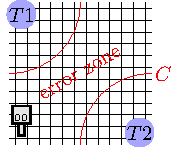
\includegraphics[width=0.5\linewidth]{robotgrid.pdf} 
\label{robotgridfig}
\end{figure}

We consider now that, 
in reality (thus here for the simulations),
and contrary to what is described by the model, 
the image processing algorithms badly perform 
when the robot is far away from targets, 
\textit{i.e.}, if $\forall i \in \{1,2\}$, 
$\sqrt{(x-x_i)^2+(y-y_i)^2}>C$, 
with $C$ a positive constant, then
$\textbf{p} \paren{good_i \sachant x,y } = 1-P_{bad} < \frac{1}{2}$.  
In all other cases, we assume that 
the probabilistic model is the good one. 
Figure \ref{robotgridfig} illustrates this problem,
and indicates the zone where the robot misperceives
calling it ``error zone''.
For the following numerical experiments,
we used $10^4$ simulations to compute 
the statistical mean of the total reward at execution. 
The grid was $10 \times 10$, $D=10$ and $C=4$. 

Figure \ref{figureexp}.a shows that the probabilistic model 
is more affected by the introduced error than the possibilistic one: 
it shows the total reward at execution of each model as a function of $P_{bad}$, 
the probability of badly observing targets 
when the robot's location is such that 
$\sqrt{(x-x_i)^2+(y-x_i)^2} >C$,
\textit{i.e.} when the robot is in the ``error zone''. 
This is due to the fact that the possibilistic update 
of the belief state does not take into account new observations 
when the robot has already obtained a more reliable one, 
whereas the probabilistic model modifies the current belief at each step. 
Indeed, as there are only two hidden states ($A1$ and $A2$)
that we now denote by $s_h^1$ and $s^2_h$, 
if $\beta_{h}(s_{h}^1)<1$, then $\beta_{h}(s_{h}^2)=1$ 
(possibilistic normalization). 
As the hidden state does not change during the mission,
the joint possibility distribution
over the hidden state and the observation 
is the minimum of the possibility distribution over the system state
(described by the current belief state) 
and the observation possibility degree:
e.g. for $s_h^1$, the joint distribution is 
$\min \set{ \pi \paren{ o_h \sachant s_v,s_h^1, a}, \beta_h(s_h^1)  }$,
with $o_h \in \set{ oAA,oAB,oBA,oBB}$.
It implies that the joint possibility of $s_{h}^1$ 
and the observation $o_h$, 
is smaller than $\beta_{h}(s_{h}^1)$. 
The possibilistic counterpart of the belief update equation,
see the equation (\ref{possbeliefupdate}) or the equation (\ref{equation_piMOMDPupdate})
for Mixed-Observability settings, 
ensures that the next belief is either more skeptic about $s_{h}^1$ 
if the observation is more reliable and confirms the prior belief 
($\pi \paren{o_h \sachant s_v,s_h^1,a }$ is smaller than $\beta_{h}(s_{h}^1)$); 
or changes to the opposite belief 
if the observation is more reliable and contradicts 
the prior belief 
($\pi \paren{o_h \sachant s_v,s_h^2,a }$ is smaller than both $\beta_{h}(s_{h}^1)$ and $\pi \paren{o_h \sachant s_v,s_h^1,a }$); 
or yet simply remains unchanged 
if the observation is not more 
informative than the current belief. 

The following theorem gives sufficient conditions
leading to an informative possibilistic belief update
\textit{i.e.} which make the resulting belief state
more specific (see Definition \ref{def_specificity} of Section \ref{posspres}) 
than the previous one:
a belief state $\beta_1 \in \Pi^{\mathcal{S}}_{\mathcal{L}}$ 
is said more specific than a belief state $\beta_2 \in \Pi^{\mathcal{S}}_{\mathcal{L}}$
if $\forall s \in \mathcal{S}$, $\beta_1(s) \leqslant \beta_2(s)$.
In order to get a total order on $\Pi^{\mathcal{S}}_{\mathcal{L}}$,
the ranking relation $\preceq$ is defined to
sort belief states with respect to their specificity:
\[\beta_1 \preceq \beta_2 \Leftrightarrow \sum_{s \in \mathcal{S}} \beta_1(s) \leqslant \sum_{s \in \mathcal{S}} \beta_2(s).  \]
Note that if $\beta_1$ is more specific than $\beta_2$, 
then $\beta_1 \preceq \beta_2$.

\begin{theorem}[Conditions for an increasing specificity of the belief states]
\label{theorem_specificity_belief}
Let $\beta_0 \in \Pi^{\mathcal{S}}_{\mathcal{L}}$ 
be the initial belief state modeling the total ignorance
\textit{i.e.} $\forall s \in \mathcal{S}$, $\beta_0(s)=1$.
If the transition function $\pi \paren{ s' \sachant s, a }$ 
is deterministic,
and if the observations are not informative, 
\textit{i.e.} $\forall s' \in \mathcal{S}$ , $\forall a \in \mathcal{A}$, $\forall o' \in \mathcal{O}$, $\pi \paren{o' \sachant s',a}=1$,
then $\beta_{t+1} \preceq \beta_{t}$,
where $\beta_{t+1} \in \Pi^{\mathcal{S}}_{\mathcal{L}}$ 
is the result of an update (\ref{possbeliefupdate}) of the belief state 
$\beta_t \in \Pi^{\mathcal{S}}_{\mathcal{L}}$, 

The result $\beta_{t+1} \preceq \beta_{t}$
remains true
if, for each action $a \in \mathcal{A}$,
the transition possibility distributions 
$\pi \paren{s' \sachant s,a  } = \mathds{1}_{\set{s=s'}}$
(\textit{i.e.} is equal to $1$ if $s'=s$ and $0$ otherwise),
and $\forall o' \in \mathcal{O}$, $\forall a \in \mathcal{A}$,
$\forall s', \tilde{s} \in \mathcal{S}$, 
$\pi \paren{o' \sachant s',a} \neq \pi \paren{ o' \sachant \tilde{s}, a }$.
\end{theorem}
The proof is given in Annex \ref{theorem_specificity_belief_RETURN}.
Note that this theorem was devoted to $\pi$-POMDP.
However, the same result holds for $\pi$-MOMDPs,
replacing $s \in \mathcal{S}$ by $s_h \in \mathcal{S}_h$ and $o \in \mathcal{O}$ by $o_h \in \mathcal{O}_h$. 
Note also that the conditioning 
presented in Definition \ref{altern_qual_cond} of Section \ref{qualitative_indep}
leads to another belief update:
with this one, if $\beta_{t+1}$ is the update of the belief state $\beta_t$,
$\beta_{t+1}$ is not less specific than $\beta_t$. 
However, it does not ensure that $\beta_{t+1} \preceq \beta_t$.

The probabilistic belief update does not have these capabilities 
to directly change to the opposite belief and to disregard less reliable observations: 
the robot then proceed towards the wrong target because 
it is initially far away and thus badly observes targets
(without knowing it). 
When it is close to this target, 
it gets good observations and gradually modifies its belief 
which becomes true enough to convince it to go towards the right target. 
However it has to cross a remote area away from targets: 
this yet gradually modifies its belief, 
which becomes wrong, 
and the robot finds itself 
in the same initial situation: 
it loses thus a lot of time 
to get out of this loop. 
We can observe that the total reward increases 
for high probabilities of misperceiving $P_{bad}$: 
this is because this high error 
leads the robot to reach 
the wrong target faster, 
thus to entirely know that 
the true target is the other one.
\begin{figure}\centering
\begin{tabular}{cc}
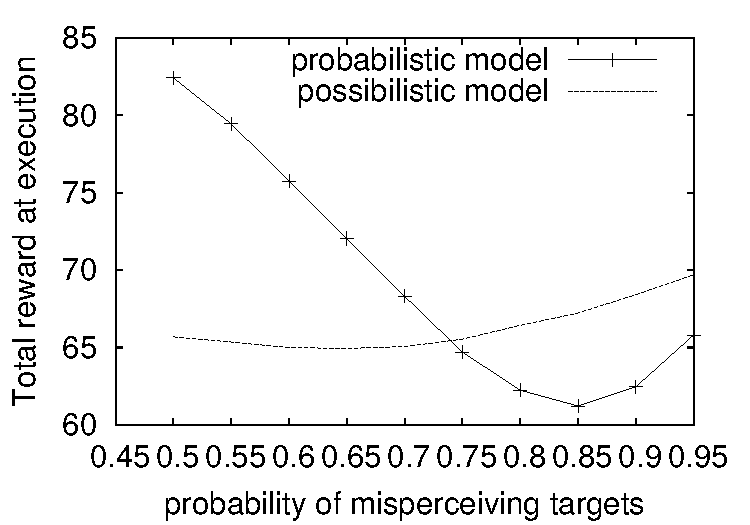
\includegraphics[width=.45\linewidth]{courbe1.pdf} &
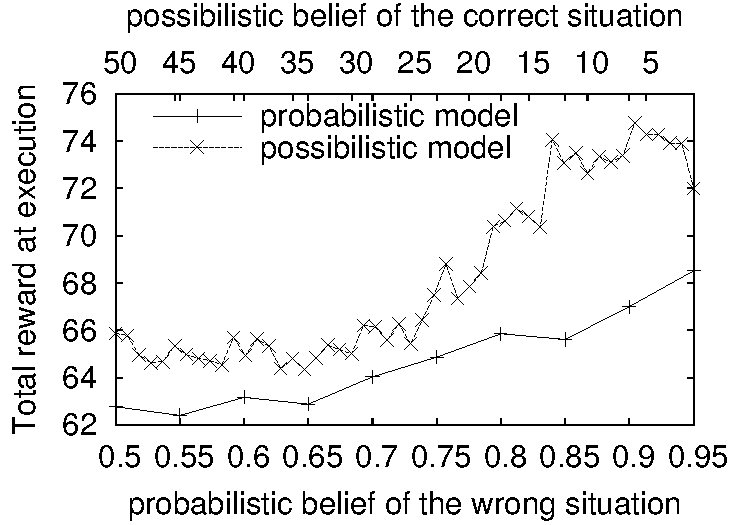
\includegraphics[width=.45\linewidth]{courbe2.pdf} \\
(a) Varying $P_{bad}$.  & (b) Varying $\beta_0$: here $\mathcal{L}=\set{0,1,\ldots,50}$.
\end{tabular}
\caption{Comparison of the total reward gathered at execution for possibilistic and probabilistic models.} \label{figureexp}
\end{figure}

%% IKI TODO

Now if we set $P_{bad}=0.8$ 
and evaluate the total reward 
at execution for different 
wrong initial belief states, 
we get Figure \ref{figureexp}.b 
with the same parameters: 
we compare here the possibilistic model 
and the probabilistic one 
when the initial belief state 
is strongly oriented 
towards the wrong hidden states 
(i.e. the agent strongly 
believes that target 1 is B 
whereas it is A in reality). 
Note that the possibilistic belief state 
of the good target 
decreases when the necessity of the
bad one increases. 
This figure shows that the possibilistic model 
yields higher rewards at execution 
if the initial belief state is wrong 
and the observation function is imprecise~\footnote{
The implementation of the solver,
as well as a generator of descriptions of such recognition problems
(expressed in the RDDL language \cite{Sanner_relationaldynamic}) 
which is the input of the solver,
are available on the repository \url{https://github.com/drougui/ppudd}~:
executions can be simulated using the possibilistic optimal strategy
which is the output of the solver.}.
%\subsection{Possibilistic Belief Process}
%conditionnement 2!\\
%\section{Study of Alternative Criteria + conditionnement 2}

\section{Conclusion}
We have proposed a Value Iteration algorithm for possibilistic MDPs, which
can produce optimal stationary strategies in infinite horizon contrary to previous
methods. We have provided a complete proof of convergence that relies on the
existence of intermediate ``stay'' actions that vanish 
for non goal states in the final optimal strategy. 
Finally, we have extended this algorithm to a new Mixed-Observable
possibilistic MDP model, whose complexity is exponentially smaller than
possibilistic POMDPs, so that we could compare $\pi$-MOMDPs with their
probabilistic counterparts on realistic robotic problems. Our experimental
results show that possibilistic strategies can outperform probabilistic 
ones when the probabilities of the observation function are not precisely known,
and thus defined quite differently from the actual ones.

A value iteration algorithm for the pessimistic $\pi$-MDPs 
can be easily written on the basis of the optimistic value iteration algorithm,
Algorithm \ref{algorithmIVPIMDP}.
However, the optimality of the returned strategy seems 
hard to prove, essentially because it is not enough 
to construct a maximizing trajectory, 
as the proof in Annex \ref{proofThmIV} does. 
The works \cite{LIP61498,DBLP:books/daglib/0024909} 
may be useful materials to help us to get results about pessimistic 
$\pi$-MDP in infinite horizon settings.

Note that, if some probabilistic information 
is really known by the designers of the model,
the $\pi$-POMDP is a qualitative approximation
of the probabilistic POMDP: in such cases
the quantitative information which is available
is not taken into account, in order to simplify 
the problem resolution.
Indeed, this model only implies maximum and minimum operators.
Note also that if the model has been built from expert 
qualitative information about the plausible behaviour of the system,
an arbitrary probabilistic POMDP offers no more guarantee than
the possibilistic one 
which only uses really available description of the problem.

Finally, as highlighted by the experiment,
while the $\pi$-POMDPs are
based on a computationally simpler uncertainty model 
than the probabilistic POMDP,
the possibilistic belief updating process may 
has an interesting behaviour.
Under some sufficient assumptions
given by Theorem \ref{theorem_specificity_belief},
the belief state is not modified 
by less reliable information
than the previously gathered information, 
but is able to change to a quite opposite belief state
if an information item which suggests it and which is more reliable is received.
More complex problems have to be studied 
to get a better overview of this behavior
in a wider set of situations.
However, $\pi$-POMDPs with a large system state
(or $\pi$-MOMDPs with large $\mathcal{S}_h$) 
cannot be solved with reasonable computation times 
by algorithms developed until now.
The next chapter presents and uses another problem structure,
the possibilistic counterpart of \textit{factored POMDPs},
which leads to easier computations of optimal possibilistic strategies 
and making various experiments:
the developed solvers use Algebraic Decision Diagrams
avoiding some useless computations
and making handled data more compact.
